\documentclass[11pt,a4paper]{article}

% ===== 中文支持 =====
\usepackage[UTF8,scheme=plain]{ctex}

% ===== 数学包 =====
\usepackage{amsmath,amssymb,amsthm,mathtools}
\usepackage{bm}

% ===== 排版 =====
\usepackage[margin=1in]{geometry}
\usepackage{enumitem}
\usepackage{hyperref}
\usepackage{xcolor}
\usepackage{tcolorbox}
\usepackage{listings}
\usepackage{caption}
\usepackage{tikz}
\usetikzlibrary{arrows.meta, calc, decorations.markings, positioning}

\hypersetup{colorlinks=true, linkcolor=blue!50!black, citecolor=blue!50!black, urlcolor=blue!50!black}

% ===== 自定义环境 =====
\newtheoremstyle{mythm}{8pt}{8pt}{\itshape}{}{\bfseries}{：}{ }{}
\theoremstyle{mythm}
\newtheorem{theorem}{定理}[section]
\newtheorem{lemma}[theorem]{引理}
\newtheorem{proposition}[theorem]{命题}
\newtheorem{corollary}[theorem]{推论}

\newtheoremstyle{mydef}{8pt}{8pt}{}{}{\bfseries}{：}{ }{}
\theoremstyle{mydef}
\newtheorem{definition}[theorem]{定义}
\newtheorem{example}[theorem]{例子}
\newtheorem{remark}[theorem]{注记}
\newtheorem{exercise}[theorem]{练习}

\sloppy

% ===== 数学符号宏 =====
\newcommand{\R}{\mathbb{R}}
\newcommand{\E}{\mathbb{E}}
\newcommand{\tr}{\operatorname{tr}}
\newcommand{\diag}{\operatorname{diag}}
\newcommand{\rank}{\operatorname{rank}}
\newcommand{\sign}{\operatorname{sign}}
\newcommand{\msign}{\operatorname{msign}}
\newcommand{\mcsgn}{\operatorname{mcsgn}}
\newcommand{\inner}[2]{\langle #1, #2 \rangle}
\newcommand{\Frob}{\mathrm{F}}
\newcommand{\nuc}{\ast}
\DeclareMathOperator*{\argmin}{arg\,min}
\DeclareMathOperator*{\argmax}{arg\,max}

% ===== 代码样式 =====
\definecolor{codegray}{rgb}{0.95,0.95,0.95}
\definecolor{codekey}{rgb}{0.13,0.29,0.53}
\definecolor{codecom}{rgb}{0.30,0.55,0.30}
\definecolor{codestr}{rgb}{0.65,0.13,0.13}
\lstset{
  backgroundcolor=\color{codegray},
  basicstyle=\ttfamily\footnotesize,
  keywordstyle=\color{codekey}\bfseries,
  commentstyle=\color{codecom}\itshape,
  stringstyle=\color{codestr},
  numbers=left, numberstyle=\tiny\color{gray},
  breaklines=true, frame=single, tabsize=4,
  showstringspaces=false, language=Python
}

% ===== 文档信息 =====
\title{\textbf{流形上的最速下降}\\[6pt]
\large 优化算法专题讲义}
\author{}
\date{\today}

\begin{document}

\maketitle
\thispagestyle{empty}

\begin{abstract}
本讲义系统介绍\textbf{矩阵参数 + 流形约束}下的最速下降问题。主线是把"最小作用量原理"扩展到带等式约束的情形：先给增量加范数约束（推出 SGD、SignSGD、Muon），再给参数本身加流形约束（推出超球面 / 正交 / Stiefel / 谱球面上的 Muon）；通用求解套路是"一阶近似 + 待定系数 + 不动点迭代/对偶梯度下降"。讲义穿插具体的低维数值算例，最后给出可在课堂演示的 NumPy 参考代码。

\medskip
\noindent\textbf{先修}：矩阵分析（SVD、谱范数、核范数）、凸优化（拉格朗日乘子、Hölder 不等式）、深度学习常用优化器。

\noindent\textbf{贯穿主线}：$\min_{\Delta W} L(W+\Delta W)$ s.t.\ $\rho(\Delta W)\le \eta$，并对参数 $W$ 添加约束 $\mathcal{M}(W)=0$。
\end{abstract}

\tableofcontents
\newpage

% ============================================================
\section{引入：为什么要研究流形上的最速下降？}
% ============================================================

在深度学习训练中，对参数 $W$ 施加额外约束的需求并不少见：
\begin{itemize}[leftmargin=2em]
    \item \textbf{超球面约束} $\|w\|_2 = 1$：归一化方向向量、prototype-based 分类、speaker embedding。
    \item \textbf{正交约束} $W^\top W = I$：稳定的 RNN/SSM 转移矩阵、归一化流、防止表示坍缩、LoRA 的去冗余参数化。
    \item \textbf{Stiefel 约束} $W^\top W = I_m$（$W \in \R^{n\times m}$，$n>m$）：半正交投影矩阵。
    \item \textbf{谱范数约束} $\|W\|_2 = 1$：Lipschitz 控制、谱归一化 GAN、稳定训练。
\end{itemize}
这一类问题传统上用 Riemannian SGD 求解，但流形上的指数映射往往昂贵。本讲义采用一种近期更为实用的视角——把约束\emph{统一}进"最小作用量原理"：\textbf{先求最速下降方向 $\Phi$，再做回缩 (retraction) 把参数拉回流形}。该视角在 Muon 优化器\cite{muon} 和 \emph{Orthogonal Manifold} \cite{bernstein-orth} 中得到了系统应用。

% ============================================================
\section{第一讲：最速下降的统一框架}\label{sec:framework}
% ============================================================

\subsection{最小作用量原理}

设损失为 $L(\cdot)$，参数为 $w$，更新量为 $\Delta w$。一个"好"的优化器应当\textbf{又稳又快}：在一定步长内使损失下降最多。形式化为：
\begin{equation}\label{eq:min-action}
\min_{\Delta w}\; L(w+\Delta w)
\qquad
\text{s.t.}\;\; \rho(\Delta w)\le \eta
\end{equation}
其中 $\rho$ 是衡量"步子"大小的某种范数。$\rho$ 的不同选择对应不同优化器。

\subsection{一阶近似下的方向问题}

当 $\eta$ 充分小，做一阶展开 $L(w+\Delta w)\approx L(w)+\inner{g}{\Delta w}$，$g=\nabla L(w)$。代入并令 $\Delta w = -\kappa\,\varphi$、$\rho(\varphi)=1$，可得等价目标：
\begin{equation}\label{eq:direction}
\boxed{\quad\max_\varphi\; \inner{g}{\varphi}\quad \text{s.t.}\;\; \rho(\varphi)=1\quad}
\end{equation}
此即"最速下降方向"问题。$\varphi$ 的反方向就是损失下降最快的方向；该方向\textbf{依赖于 $\rho$ 的选择}。

\subsection{若干基本范数下的最速下降}

\begin{example}[$L^2$ 范数：朴素 SGD]
当 $\rho(\varphi) = \|\varphi\|_2$，由柯西不等式 $\inner{g}{\varphi}\le \|g\|_2$，等号在 $\varphi \propto g$ 取得，故
$\varphi^\ast = g/\|g\|_2$，$\Delta w = -\eta\,g/\|g\|_2$。这正是规范化梯度下降。
\end{example}

\begin{example}[$L^p$ 范数：pbSGD]
$\rho(\varphi) = \|\varphi\|_p$，由 Hölder 不等式 $\inner{g}{\varphi}\le \|g\|_q\|\varphi\|_p$（$1/p+1/q=1$）。等号条件 $\varphi^{[p]} \propto g^{[q]}$，其中 $g^{[\alpha]}_i := \sign(g_i)\,|g_i|^\alpha$，解得
$\varphi^\ast = g^{[q/p]}/\|g^{[q/p]}\|_p$。
两个特例：$p=2$ 退化为 SGD；$p\to\infty$ 时 $q\to 1$，$\varphi^\ast = \sign(g)$，即 SignSGD。
\end{example}

\begin{remark}
$\rho$ 是优化器中很本质的\textbf{先验} (inductive bias)。把它从 $L^2$ 推广到\emph{矩阵的谱范数}，正是 Muon 的来历——也是本讲义的真正起点。
\end{remark}

% ============================================================
\section{第二讲：流形上的几何语言}\label{sec:geom}
% ============================================================

在进入 Muon 与流形约束之前，先把后面要反复使用的几何概念厘清：\textbf{内蕴/外蕴视角、流形、切空间、测地线、回缩}。本讲也用一个 NLP 中的具体应用例子说明"测地线距离"的实用价值。

\subsection{内蕴几何与外蕴几何}\label{sec:intrinsic}

进入形式定义之前，先把一个本质区分讲清楚——\textbf{同一个流形可以从两种视角看}：

\begin{itemize}[leftmargin=2em]
\item \textbf{外蕴 (extrinsic) 视角}：把流形看成嵌在某个大空间里的子集，关心它"长什么样"——形状、位置、坐标。
\item \textbf{内蕴 (intrinsic) 视角}：只用流形内部能"摸到"的东西——长度、角度、面积——\emph{不引用流形外部的方向或坐标}。
\end{itemize}

\paragraph{画面 1：圆筒 $=$ 平纸（内蕴上）}
把 A4 纸卷成圆筒（不撕、不拉伸）。外蕴上完全不同（一平一弯）；内蕴上完全相同——纸面上画的所有距离、角度、三角形面积，卷起来后一个都没变。住在纸上的蚂蚁感觉不到任何差别。

\paragraph{画面 2：蚂蚁 vs 人的距离观}
球面上的对径两点 $p, q$：
\begin{itemize}[leftmargin=2em]
\item 外蕴距离 $\|p-q\| = 2R$：穿过球心的直线段——蚂蚁走不了。
\item 内蕴距离 $d_g(p,q) = \pi R$：沿大圆走的最短弧——蚂蚁实际能走的最短路径。
\end{itemize}

\subsubsection*{度量张量 $g_{ij}$：把内蕴几何形式化}

\textbf{光说"蚂蚁能测量的东西"还不够形式化}。怎么把"住在面上能感知到的几何"写成数学？答案是给每点的切空间装一个内积——这个东西就叫 \textbf{Riemann 度量 (Riemannian metric)} 或\textbf{度量张量 $g_{ij}$}。

\textbf{定义}：在每点 $p \in \mathcal{M}$ 的切空间 $T_p\mathcal{M}$ 上选一个内积 $\langle \cdot, \cdot \rangle_p$，使其随 $p$ 光滑变化。在局部坐标 $(x^1, \dots, x^n)$ 下，
$$g_{ij}(p) := \langle \partial_i, \partial_j\rangle_p,$$
即坐标基向量的两两内积。$g_{ij}$ 是一个对称正定矩阵（依赖 $p$）。

\textbf{有了 $g_{ij}$ 就有所有内蕴几何}：
\begin{itemize}[leftmargin=2em]
\item 切向量 $u = u^i \partial_i$ 的长度：$\|u\|^2 = g_{ij} u^i u^j$。
\item 两个切向量的夹角：$\cos\alpha = g_{ij} u^i v^j / (\|u\|\|v\|)$。
\item 曲线 $\gamma$ 的弧长：$L = \int \sqrt{g_{ij}\dot x^i \dot x^j}\, dt$（这正是 §\ref{sec:geodesic-eq} 的弧长泛函）。
\item 面积元：$dA = \sqrt{\det g}\, dx^1 \cdots dx^n$。
\item 测地线、Christoffel 符号、曲率——全都从 $g_{ij}$ 及其导数算出。
\end{itemize}

\begin{tcolorbox}[colback=blue!3,colframe=blue!50!black]
\textbf{度量张量 $g_{ij}$ 完全决定了流形的内蕴几何}。两个流形若存在坐标使它们的 $g_{ij}$ 相同，蚂蚁就分不清自己住在哪一个上——它们\textbf{内蕴等同 (isometric)}。
\end{tcolorbox}

\textbf{嵌入流形的诱导度量}：若 $\mathcal{M} \subset \R^N$ 由参数 $\mathbf{r}(x^1,\dots,x^n)$ 给出，则继承自 $\R^N$ 的内积自动给出度量
$$g_{ij} = \big\langle \partial_i \mathbf{r},\, \partial_j \mathbf{r}\big\rangle_{\R^N}.$$
这就是经典曲面论里的"\textbf{第一基本形式}"。

\subsubsection*{算例 1：球面}
$\mathbf{r}(\theta, \phi) = R(\sin\theta\cos\phi,\,\sin\theta\sin\phi,\,\cos\theta)$。算偏导内积（用 SymPy 符号验过）：
$$g_{\theta\theta} = R^2,\quad g_{\phi\phi} = R^2\sin^2\theta,\quad g_{\theta\phi} = 0.$$
即
$$g = \begin{pmatrix}R^2 & 0\\ 0 & R^2\sin^2\theta\end{pmatrix},\qquad ds^2 = R^2\,d\theta^2 + R^2\sin^2\theta\,d\phi^2.$$

\textbf{用 $g_{ij}$ 算东西}（$R=1$）：
\begin{itemize}[leftmargin=2em]
\item 北纬 $30°$ 圆周长（$\theta = \pi/3$ 固定）：$\int_0^{2\pi}\sqrt{\sin^2(\pi/3)}\,d\phi = 2\pi\sin(\pi/3) \approx 5.44$。
\item 赤道周长（$\theta = \pi/2$）：$2\pi\sin(\pi/2) = 2\pi \approx 6.28$。
\end{itemize}
两个数都跟外蕴坐标无关，纯由 $g_{ij}$ 决定。

\subsubsection*{算例 2：圆筒 = 平面（内蕴）的代数证明}
$\mathbf{r}(u, v) = (R\cos u,\, R\sin u,\, v)$。算诱导度量：
$$g_{uu} = R^2,\quad g_{vv} = 1,\quad g_{uv} = 0\quad\Longrightarrow\quad ds^2 = R^2\,du^2 + dv^2.$$
做坐标变换 $u' = R u$（弧长参数化）：
$$ds^2 = du'^2 + dv^2 \quad\Longleftrightarrow\quad g_{i'j'} = \begin{pmatrix}1 & 0\\ 0 & 1\end{pmatrix}.$$
这\textbf{完全等同于平面}的度量！所以\textbf{圆筒和平面内蕴等同}——上一节"卷纸"的直觉，到这里有了精确的代数表述：在合适坐标下度量张量\emph{逐点完全相同}。蚂蚁的所有测量结果都不会区分两者。

\subsubsection*{Theorema Egregium：$g_{ij}$ 决定一切}

球面的"弯曲度"由\textbf{高斯曲率} $K$ 衡量。它\textbf{看起来}是个外蕴量——经典定义用第二基本形式（描述曲面如何在 $\R^3$ 中弯）。但 Gauss 在 1827 年证明了一件惊人的事：$K$ \textbf{只依赖 $g_{ij}$ 及其导数}，与嵌入方式无关。具体公式（正交坐标 $g_{12} = 0$ 时的 \textbf{Brioschi 公式}）：
\begin{equation}\label{eq:brioschi}
K = -\frac{1}{2\sqrt{EG}}\!\left[\partial_v\!\left(\frac{\partial_v E}{\sqrt{EG}}\right) + \partial_u\!\left(\frac{\partial_u G}{\sqrt{EG}}\right)\right],\quad E = g_{11},\;G = g_{22}.
\end{equation}

\begin{theorem}[Theorema Egregium]
高斯曲率 $K$ 是\textbf{内蕴量}：仅由度量张量 $g_{ij}$ 决定。
\end{theorem}

\textbf{算例验证}（用 SymPy 符号验过）：

\textbf{(a) 球面} $g = \diag(R^2, R^2\sin^2\theta)$：$E = R^2, G = R^2\sin^2\theta$，$\sqrt{EG} = R^2\sin\theta$。
\begin{itemize}[leftmargin=2em]
\item $\partial_\phi E = 0$，第一项消失。
\item $\partial_\theta G = 2R^2\sin\theta\cos\theta$，故 $\partial_\theta G / \sqrt{EG} = 2\cos\theta$。
\item $\partial_\theta(2\cos\theta) = -2\sin\theta$。
\item 合起来 $K = -\frac{1}{2 R^2\sin\theta}\cdot(-2\sin\theta) = \boxed{\frac{1}{R^2}}.$
\end{itemize}
跟外蕴定义算出的 $K = 1/R^2$ \textbf{完全一致}——而且整个推导没碰过 $\R^3$ 的"球内一点"。

\textbf{(b) 圆筒} $g = \diag(R^2, 1)$：所有度量分量都是常数，所有偏导都是零，故 $K = 0$。

\textbf{(c) 平面（极坐标）}$g = \diag(1, \rho^2)$：算下来也是 $K = 0$。

\medskip
\textbf{对比}：在 $\R^3$ 里看，圆筒"明明是弯的"（视觉上），但 $K = 0$ 跟平面一样——因为可以\emph{展开}成平面。而球面 $K = 1/R^2 > 0$ 不能展开（你不可能把橘子皮压平而不撕裂）。这就是为什么\textbf{地图必失真}（球面到平面没有保距映射）——这件事 Gauss 的定理给出了精确的内蕴判据。

\subsubsection*{对优化的启示}

讲义后面把这个抽象图式翻译到优化语言：
\begin{itemize}[leftmargin=2em]
\item \textbf{最速下降方向}的"几何"由切空间上的\textbf{度量}决定。换种度量 = 换种"最速"——
$$\rho(\Delta\theta) = \sqrt{(\Delta\theta)^\top G(\Delta\theta)},\qquad G\;\text{由优化器选择}.$$
SGD 取 $G = I$（欧氏度量），natural gradient 取 $G = F$（Fisher 度量），Muon 隐式取的是谱范数对应的"算子度量"。
\item \textbf{Fisher 信息 $F$ 就是分布流形的 Riemannian 度量 $g_{ij}$}。这不是类比——上面提到 $F(\theta') = J^\top F(\theta) J$ 严格按 $g_{ij}$ 张量变换规律。
\item \textbf{曲率（Hessian 减去预条件项）} 在最优化里对应"下降方向被流形扭曲多少"——但这是另一层故事，工程上常用对角/块对角近似处理。
\end{itemize}

\begin{remark}[历史插话]
Gauss 把这条结果命名为 \emph{Theorema Egregium}（拉丁文"绝妙定理"）——是他个人觉得最得意的工作。它直接孕育了黎曼几何、爱因斯坦广义相对论（时空的几何由内蕴度量决定）、以及今天的流形学习与流形优化。下次你看到 Adam 的 $\hat v_t \propto F$ 估计、自然梯度的 $F^{-1}$、Riemannian SGD 的切空间投影——它们的代数根都在这条 200 年前的定理上。
\end{remark}

\subsubsection*{参数化的歧义}

更深一步：\textbf{同一个流形，用不同参数描述时，"看起来"完全不同}。

\begin{example}[同一条曲线的两种参数化]\label{ex:circle-param}
单位圆 $\mathcal{M} = \{(x,y): x^2+y^2 = 1\}$ 可以这样参数化：
\begin{itemize}[leftmargin=2em]
\item $\phi_1(t) = (\cos t,\, \sin t)$，$t \in [0, 2\pi)$——\emph{等速}画圆；
\item $\phi_2(s) = (\cos(s^3),\, \sin(s^3))$，$s \in [0, (2\pi)^{1/3})$——\emph{非等速}：$s$ 接近 $0$ 时跑得慢，接近 $(2\pi)^{1/3}$ 时跑得快。
\end{itemize}
图像（点集）完全相同；但在 $t$ 坐标和 $s$ 坐标里，"参数走一步 $\Delta = 0.1$"对应的圆上弧长差异巨大。\textbf{同一个流形，参数空间里的几何完全不同}。

\textbf{优化的视角}：在参数空间做"梯度下降等距前进"，到底是在流形上等距，还是在参数空间等距？取决于参数化——这件事并不显然。
\end{example}

\subsubsection*{Hessian 是外蕴的，Fisher 是内蕴的}

把这件事在优化里说精确。考虑损失 $L(\theta)$，做参数变换 $\theta = \phi(\theta')$，记 Jacobian $J = \partial\theta/\partial\theta'$。

\textbf{梯度变换}：$\nabla_{\theta'} L = J^\top \nabla_\theta L$——像协变向量一样变换，干净。

\textbf{Hessian 变换}：
\begin{equation}\label{eq:hess-transform}
\nabla^2_{\theta'} L \;=\; J^\top (\nabla^2_\theta L)\, J \;+\; \sum_i (\partial_i L)\,\nabla^2_{\theta'}\phi_i.
\end{equation}
后一项一般\textbf{不为零}——这正是"非线性参数化引入的额外曲率项"。所以 Hessian \textbf{依赖参数化}，不是流形上的内蕴量。

例外是临界点 $\nabla_\theta L = 0$ 处，第二项消失，Hessian 像 $(0,2)$-张量一样变换——这是为什么 Morse 引理等理论结果只在临界点附近成立。

\textbf{Fisher 信息则完全不同}。对似然模型 $p_\theta(x)$，
$$F(\theta) := \E_x\!\left[\nabla_\theta \log p_\theta\,\nabla_\theta \log p_\theta^\top\right].$$
做参数变换，由链式法则
\begin{equation}\label{eq:fisher-transform}
F(\theta') \;=\; J^\top F(\theta)\, J
\end{equation}
\textbf{没有第二项}——因为 $\E[\nabla\log p_\theta] = 0$，相当于"在期望意义下永远处于临界点"。\eqref{eq:fisher-transform} 恰是 Riemann 度量张量在坐标变换下的标准行为。所以\textbf{$F$ 在分布流形 $\mathcal{M} = \{p_\theta\}_\theta$ 上定义了一个内蕴 Riemann 度量}：同一个分布，无论怎么参数化，它在 $\mathcal{M}$ 上的几何都一样。

\textbf{这正是 natural gradient 的来源}：
$$\Delta\theta = -\eta\, F(\theta)^{-1}\nabla_\theta L$$
是参数化无关的更新方向——换一种参数，在\emph{分布空间}里走过的路径不变。

\subsubsection*{具体数值算例：Hessian 跑偏，Fisher 守恒}

为了把上面抽象的张量公式落到实处，看一个最小的算例。

\textbf{设置}：模型 $p_\mu(x) = \mathcal{N}(\mu, 1)$，损失 $L(\mu) = -\log p_\mu(x_0) = \tfrac{1}{2}(x_0-\mu)^2 + c$，观测 $x_0 = 2$。重参数化 $\mu = \phi(\theta) := \theta^3$。比较点 $\mu = 1$（即 $\theta = 1$）。

\textbf{第 1 步：在 $\mu$ 坐标下直接算}
\begin{align*}
\nabla_\mu L &= -(x_0 - \mu) = -1, & \nabla^2_\mu L &= 1, \\
F(\mu) &= \E_x[(x-\mu)^2] = 1 & &\text{（$\mathcal{N}(\mu,1)$ 的方差）}.
\end{align*}

\textbf{第 2 步：在 $\theta$ 坐标下直接算}
$L(\theta) = \tfrac{1}{2}(x_0 - \theta^3)^2 + c$，求导得
\begin{align*}
\nabla_\theta L &= -3\theta^2(x_0 - \theta^3) = -3, \\
\nabla^2_\theta L &= -6\theta(x_0 - \theta^3) + 9\theta^4 = -6 + 9 = \boxed{3}.
\end{align*}
另外 $\nabla_\theta \log p = 3\theta^2(x-\theta^3)$，故
$$F(\theta) = \E_x[(3\theta^2)^2(x-\theta^3)^2] = 9\theta^4 \cdot 1 = \boxed{9}.$$

\textbf{第 3 步：用变换公式核对}
$J = d\mu/d\theta = 3\theta^2 = 3$，$\phi'' = 6\theta = 6$。

\emph{Hessian 公式 \eqref{eq:hess-transform}}：
$$\nabla^2_\theta L \stackrel{?}{=} J^2\nabla^2_\mu L + (\nabla_\mu L)\phi'' = 9\cdot 1 + (-1)\cdot 6 = 9 - 6 = 3.\quad\checkmark$$
注意$\boxed{-6}$这个第二项——它就是"非线性参数化引入的额外项"。

\emph{Fisher 公式 \eqref{eq:fisher-transform}}：
$$F(\theta) \stackrel{?}{=} J^2 F(\mu) = 9\cdot 1 = 9.\quad\checkmark$$
\textbf{没有第二项}。

\textbf{第 4 步：意义对比表}

\begin{center}
\begin{tabular}{l|cccc}
\hline
量 & $\mu$ 坐标 & $\theta$ 坐标 & 张量纯变换预测 & 额外项 \\\hline
Hessian & $1$ & $3$ & $9$（不对！） & $-6$ \\
Fisher  & $1$ & $9$ & $9$（对） & $0$ \\
\hline
\end{tabular}
\end{center}

\textbf{解读}：Hessian 在两套坐标里给出的"曲率"不只差一个 Jacobian 因子——还多出来一个 $-6$，**这部分信息完全来自 $\phi$ 的非线性，与流形本身无关**。Fisher 不会，$1\to 9$ 是干净的张量变换，正是 Riemann 度量该有的行为。

\textbf{第 5 步：参数化无关性测试}

到这里我们已经看到 Hessian 跟 Fisher 在两套坐标里数值不同（$\{1,3\}$ vs $\{1, 9\}$），但还没看出"这件事在优化里到底意味着什么"。下面的测试把这个意义具象化。

\subparagraph{核心问题}
\textbf{同一个分布 $\mathcal{N}(\mu, 1)$ 朝目标 $x_0$ 的更新，在 $\mu$ 坐标和 $\theta$ 坐标里各跑一步 SGD，会得到同一个"实际更新"吗？}

更具体：分布是真实的对象，参数只是它的一种"标记方式"。用不同标记跑同一个算法，按理应给出同一个新分布——否则算法就被参数化\textbf{绑架}了，是工程师选择带来的人为伪影。

\subparagraph{怎么比较}
$\Delta\mu$（分布空间里的步）和 $\Delta\theta$（参数空间里的步）单位不同，不能直接放一起比。要做苹果对苹果的比较，必须翻译到\textbf{同一个空间}。我们选\textbf{分布空间} $\mu$ 作为公共比较场所：
\begin{itemize}[leftmargin=2em]
\item $\mu$ 坐标的更新 $\Delta\mu$：本来就在分布空间，照搬。
\item $\theta$ 坐标的更新 $\Delta\theta$：通过链式法则一阶展开
$$\Delta\mu_{\text{induced}} := J\cdot\Delta\theta = 3\Delta\theta,$$
即 $\theta$ 走 $\Delta\theta$ 时，$\mu$ \emph{实际}发生的（一阶）变化。
\end{itemize}

\textbf{$\Delta\mu$ vs $\Delta\mu_{\text{induced}}$ 是否相等}\;$\Longleftrightarrow$\;\textbf{算法是否参数化无关}。

\subparagraph{实测：普通 SGD（$\eta=1$）}
\begin{itemize}[leftmargin=2em]
\item 在 $\mu$ 下：$\Delta\mu = -\nabla_\mu L = +1$。\\
\quad（合理：分布参数从 $\mu = 1$ 朝 $x_0 = 2$ 走一步。）
\item 在 $\theta$ 下：$\Delta\theta = -\nabla_\theta L = +3$；诱导
$\Delta\mu_{\text{induced}} = 3\cdot 3 = 9$。
\end{itemize}
\begin{center}
\fbox{$\Delta\mu = 1$ vs $\Delta\mu_{\text{induced}} = 9$ \quad\Longrightarrow\quad \textbf{差 $9$ 倍，不一致}}
\end{center}
\textbf{结论}：同一个 $\eta = 1$，分布在两套坐标里实际走的距离差 $9$ 倍。SGD 的 $\eta$ 是"参数空间步长"，物理意义不稳定——\textbf{换种参数化你的优化器就变了一个}。

\subparagraph{实测：natural gradient（$\eta=1$）}
NGD 用 Fisher 的逆做预条件。
\begin{itemize}[leftmargin=2em]
\item 在 $\mu$ 下：$\Delta\mu = -F(\mu)^{-1}\nabla_\mu L = -1\cdot(-1) = +1$。
\item 在 $\theta$ 下：$\Delta\theta = -F(\theta)^{-1}\nabla_\theta L = -\tfrac{1}{9}\cdot(-3) = +\tfrac{1}{3}$；诱导
$\Delta\mu_{\text{induced}} = 3\cdot\tfrac{1}{3} = +1$.
\end{itemize}
\begin{center}
\fbox{$\Delta\mu = 1$ vs $\Delta\mu_{\text{induced}} = 1$ \quad\Longrightarrow\quad \textbf{完全一致}}
\end{center}
\textbf{结论}：NGD 在分布空间里走的步子\emph{与参数化无关}。NGD 的 $\eta$ 是"分布空间步长"，物理意义稳定——这正是上面"Fisher 是内蕴的"那句话的具体含义。

\subparagraph{为什么 NGD 能不变？}
代数上一行说清：在 $\theta$ 下，
$$\Delta\mu_{\text{induced}} = J\Delta\theta = -J F(\theta)^{-1}\nabla_\theta L = -J(J^2 F(\mu))^{-1}(J\nabla_\mu L) = -F(\mu)^{-1}\nabla_\mu L,$$
即 $\boldsymbol{F^{-1}}$\textbf{把 Fisher 变换式 $J^2 F$ 中的两个 $J$ 一起消掉}。普通 SGD 没有这一步消去，留下来的 $J$ 在不同坐标里"乱跑"，所以两条路给出不同的物理结果。

\medskip
有了这个 1D 直觉，下面把它搬到 2D 看看额外项变成矩阵后的效果。

\subsubsection*{高维算例：2D 高斯 + 非线性混合参数化}

把上面的 1D 例子搬到 2D，让 Hessian 的"额外项"成为一个真正的矩阵，看看这件事在多维里有多严重。

\textbf{设置}：
\begin{itemize}[leftmargin=2em]
\item 模型：$p_{\boldsymbol\mu}(x) = \mathcal{N}(\boldsymbol\mu, I_2)$，参数 $\boldsymbol\mu = (\mu_1, \mu_2)\in\R^2$。
\item 损失：$L(\boldsymbol\mu) = \tfrac{1}{2}\|x_0 - \boldsymbol\mu\|^2 + c$。
\item 观测：$x_0 = (3, 2)$。
\item 重参数化（\textbf{两个分量混在一起的非线性变换}）：
$$\mu_1 = \theta_1^2 + \theta_2,\qquad \mu_2 = \theta_1\,\theta_2.$$
\item 比较点：$\boldsymbol\theta = (1, 1)$，对应 $\boldsymbol\mu = (2, 1)$。
\end{itemize}

\textbf{第 1 步：在 $\boldsymbol\mu$ 坐标下}
$$\nabla_{\boldsymbol\mu} L = -(x_0 - \boldsymbol\mu) = (-1,\, -1)^\top,\quad \nabla^2_{\boldsymbol\mu} L = I_2,\quad F(\boldsymbol\mu) = I_2.$$
（Hessian 与 Fisher 都是 $I_2$，因为高斯模型 $+$ 单位协方差。）

\textbf{第 2 步：算 Jacobian 与各分量的 Hessian}
$$J = \frac{\partial \boldsymbol\mu}{\partial \boldsymbol\theta} = \begin{pmatrix} 2\theta_1 & 1\\ \theta_2 & \theta_1\end{pmatrix} = \begin{pmatrix} 2 & 1\\ 1 & 1\end{pmatrix},\quad \det J = 1.$$
$$\nabla^2 \phi_1 = \begin{pmatrix}2 & 0\\ 0 & 0\end{pmatrix},\qquad \nabla^2 \phi_2 = \begin{pmatrix}0 & 1\\ 1 & 0\end{pmatrix}.$$

\textbf{第 3 步：在 $\boldsymbol\theta$ 坐标下直接求二阶导}
设残差 $r_1 = x_{0,1} - (\theta_1^2 + \theta_2) = 1$，$r_2 = x_{0,2} - \theta_1\theta_2 = 1$。直接微分得
$$\nabla_{\boldsymbol\theta} L = \begin{pmatrix} -2\theta_1 r_1 - \theta_2 r_2\\ -r_1 - \theta_1 r_2\end{pmatrix} = \begin{pmatrix} -3\\ -2\end{pmatrix},$$
$$\nabla^2_{\boldsymbol\theta} L = \begin{pmatrix}-2r_1 + 4\theta_1^2 + \theta_2^2 & 2\theta_1 - r_2 + \theta_1\theta_2\\ 2\theta_1 - r_2 + \theta_1\theta_2 & 1 + \theta_1^2\end{pmatrix} = \boxed{\begin{pmatrix}3 & 2\\ 2 & 2\end{pmatrix}}.$$
另算 Fisher：$\nabla_{\boldsymbol\theta}\log p = J^\top(x - \boldsymbol\mu)$，故
$$F(\boldsymbol\theta) = \E\!\left[J^\top(x-\boldsymbol\mu)(x-\boldsymbol\mu)^\top J\right] = J^\top I J = J^\top J = \boxed{\begin{pmatrix}5 & 3\\ 3 & 2\end{pmatrix}}.$$

\textbf{第 4 步：用变换公式核对}

\emph{Hessian \eqref{eq:hess-transform}}：
\begin{align*}
J^\top \nabla^2_{\boldsymbol\mu} L \cdot J &= J^\top J = \begin{pmatrix}5 & 3\\ 3 & 2\end{pmatrix},\\[2pt]
\sum_i (\nabla_{\boldsymbol\mu}L)_i\, \nabla^2 \phi_i &= (-1)\!\begin{pmatrix}2 & 0\\ 0 & 0\end{pmatrix} + (-1)\!\begin{pmatrix}0 & 1\\ 1 & 0\end{pmatrix} = \boxed{\begin{pmatrix}-2 & -1\\ -1 & 0\end{pmatrix}},\\[2pt]
\text{合计} &= \begin{pmatrix}5 & 3\\ 3 & 2\end{pmatrix} + \begin{pmatrix}-2 & -1\\ -1 & 0\end{pmatrix} = \begin{pmatrix}3 & 2\\ 2 & 2\end{pmatrix}\;\checkmark
\end{align*}

\emph{Fisher \eqref{eq:fisher-transform}}：
$$F(\boldsymbol\theta) \stackrel{?}{=} J^\top F(\boldsymbol\mu)\, J = J^\top J = \begin{pmatrix}5 & 3\\ 3 & 2\end{pmatrix}\;\checkmark$$
\textbf{依然没有第二项}。

\textbf{第 5 步：意义对比}

\begin{center}
\begin{tabular}{l|cc}
\hline
量 & 张量纯变换 $J^\top M J$ & 实际 \\\hline
Hessian & $\begin{pmatrix}5 & 3\\ 3 & 2\end{pmatrix}$ & $\begin{pmatrix}3 & 2\\ 2 & 2\end{pmatrix}$（差出一个 \textbf{秩 2 的} 修正） \\[10pt]
Fisher & $\begin{pmatrix}5 & 3\\ 3 & 2\end{pmatrix}$ & $\begin{pmatrix}5 & 3\\ 3 & 2\end{pmatrix}$（一致） \\
\hline
\end{tabular}
\end{center}

\textbf{重要观察}：在 1D 情形中"额外项"只是个标量 $-6$，到 2D 它变成一个 $2\times 2$ 矩阵 $\begin{pmatrix}-2 & -1\\ -1 & 0\end{pmatrix}$。它是\textbf{满秩、非对角}的——也就是说\textbf{非线性参数化不仅会改变 Hessian 的特征值（缩放），还会改变它的特征向量（旋转坐标轴）}。优化器看到的"曲率主方向"从 $\boldsymbol\mu$ 坐标到 $\boldsymbol\theta$ 坐标，整个被参数化"扭"了一下。

\textbf{第 6 步：参数化无关性测试}

到这里我们已经看到 Hessian 跟 Fisher 在两套坐标里数值不同，但还没看出"这件事在优化里到底意味着什么"。下面的实验把这个意义具象化。

\subparagraph{核心问题}
\textbf{同一个分布模型，从 $\boldsymbol\mu$ 坐标和 $\boldsymbol\theta$ 坐标各自跑一步 SGD，会得到同一个"实际更新"吗？}

更具体地说，我们是在更新一个分布 $p_{\boldsymbol\mu}$；分布是真实的对象，参数只是它的一种"标记方式"。用不同标记方式跑同一个算法（SGD），\emph{应该}得到同一个新分布——否则算法的行为就被参数化\textbf{绑架}了，是工程师选择带来的人为伪影。

\subparagraph{怎么比较}
两条更新不能直接放一起比——一个是 $\Delta\boldsymbol\mu$（分布空间里的步），一个是 $\Delta\boldsymbol\theta$（参数空间里的步），\emph{单位都不同}。要做苹果对苹果的比较，必须把两者翻译到\textbf{同一个空间}里。我们选\textbf{分布空间} $\boldsymbol\mu$ 作为公共比较场所：
\begin{itemize}[leftmargin=2em]
\item $\boldsymbol\mu$ 坐标的更新 $\Delta\boldsymbol\mu$：本来就在分布空间，照搬。
\item $\boldsymbol\theta$ 坐标的更新 $\Delta\boldsymbol\theta$：通过链式法则一阶展开
$$\Delta\boldsymbol\mu_{\text{induced}} := J\,\Delta\boldsymbol\theta + O(\|\Delta\boldsymbol\theta\|^2),$$
即 $\boldsymbol\theta$ 走 $\Delta\boldsymbol\theta$ 时，分布参数 $\boldsymbol\mu$ \emph{实际}发生的（一阶）变化。
\end{itemize}

\textbf{两个数 $\Delta\boldsymbol\mu$ vs $\Delta\boldsymbol\mu_{\text{induced}}$ 比较的意义}：是否相等\;$\Longleftrightarrow$\;算法是否"参数化无关"。

\subparagraph{实测：普通 SGD（$\eta=1$）}
\begin{itemize}[leftmargin=2em]
\item 在 $\boldsymbol\mu$ 坐标跑 SGD：$\Delta\boldsymbol\mu = -\nabla_{\boldsymbol\mu}L = (1,\,1)^\top$。\\
\quad（直接告诉我们：分布参数应当从 $(2,1)$ 走到约 $(3,2) = x_0$，朝目标走一步——合理。）
\item 在 $\boldsymbol\theta$ 坐标跑 SGD：$\Delta\boldsymbol\theta = -\nabla_{\boldsymbol\theta}L = (3,\,2)^\top$。翻译回分布空间：
$$\Delta\boldsymbol\mu_{\text{induced}} = J\,\Delta\boldsymbol\theta = \begin{pmatrix}2 & 1\\ 1 & 1\end{pmatrix}\!\begin{pmatrix}3\\ 2\end{pmatrix} = (8,\,5)^\top.$$
\end{itemize}

\begin{center}
\fbox{\parbox{0.75\textwidth}{\centering $\Delta\boldsymbol\mu = (1,1)^\top$ \;vs\; $\Delta\boldsymbol\mu_{\text{induced}} = (8,5)^\top$ \quad$\Longrightarrow$\quad \textbf{不一致}}}
\end{center}

\textbf{结论}：\textbf{普通 SGD 不是参数化无关的}。两套坐标跑同一算法，分布空间里出来的不是同一个更新——一个朝 $(1,1)$ 走、另一个朝 $(8,5)$ 走，方向偏差大、步长差 $\sim 8\times$。换种参数化你的优化器就变了一个，这是个 bug 不是 feature。

\subparagraph{实测：natural gradient（$\eta=1$）}
NGD 用 Fisher 的逆做预条件。在 $\boldsymbol\theta$ 下 $\det F(\boldsymbol\theta) = 1$，$F^{-1} = \begin{pmatrix}2 & -3\\ -3 & 5\end{pmatrix}$。
\begin{itemize}[leftmargin=2em]
\item 在 $\boldsymbol\mu$ 坐标：$\Delta\boldsymbol\mu = -F(\boldsymbol\mu)^{-1}\nabla_{\boldsymbol\mu}L = -I\cdot(-1,-1)^\top = (1,\,1)^\top$。
\item 在 $\boldsymbol\theta$ 坐标：$\Delta\boldsymbol\theta = -F^{-1}\nabla_{\boldsymbol\theta}L = -\begin{pmatrix}2 & -3\\ -3 & 5\end{pmatrix}\!\begin{pmatrix}-3\\ -2\end{pmatrix} = (0,\,1)^\top$。翻译回分布空间：
$$\Delta\boldsymbol\mu_{\text{induced}} = J\,(0,1)^\top = \begin{pmatrix}2 & 1\\ 1 & 1\end{pmatrix}\!\begin{pmatrix}0\\ 1\end{pmatrix} = (1,\,1)^\top.$$
\end{itemize}

\begin{center}
\fbox{\parbox{0.75\textwidth}{\centering $\Delta\boldsymbol\mu = (1,1)^\top$ \;vs\; $\Delta\boldsymbol\mu_{\text{induced}} = (1,1)^\top$ \quad$\Longrightarrow$\quad \textbf{完全一致}}}
\end{center}

\textbf{结论}：\textbf{NGD 是参数化无关的}。两套坐标跑出来的更新在分布空间里看是同一个——这正是"Fisher 是内蕴度量"那句话的具体含义。

\subparagraph{为什么 NGD 能不变？}
代数上一行：在 $\boldsymbol\theta$ 下，
$$\Delta\boldsymbol\mu_{\text{induced}} = J\,\Delta\boldsymbol\theta = -J F(\boldsymbol\theta)^{-1}\nabla_{\boldsymbol\theta}L = -J(J^\top F(\boldsymbol\mu)J)^{-1}(J^\top \nabla_{\boldsymbol\mu}L) = -F(\boldsymbol\mu)^{-1}\nabla_{\boldsymbol\mu}L,$$
最后一步因为 $J(J^\top F J)^{-1}J^\top = F^{-1}$（当 $J$ 可逆时）。所以 \textbf{$F^{-1}$ 把 Fisher 变换式 $J^\top F J$ 中的两个 $J$ 一起"约掉"}——Fisher 的张量变换性质是 NGD 不变性的代数根源。普通 SGD 缺这一步消去，Jacobian 留下来"乱跑"，所以两个坐标系跑出不同步。

\paragraph{总结}
高维让"额外项是矩阵"这件事真正显形：
\begin{itemize}[leftmargin=2em]
\item Hessian 的额外项可以是\textbf{任意秩、非对角}，意味着不只是缩放，还有"旋转"——优化器以为重要的方向，其实是参数化人为造出来的方向。
\item Fisher 严格按 $J^\top F J$ 变换，是干净的内蕴张量。
\item natural gradient $F^{-1}\nabla L$ 在分布流形上的更新方向参数化无关。
\end{itemize}
这正是 Adam（对角 Fisher 近似）、K-FAC、Shampoo 这些现代优化器的几何动机：\textbf{越靠近真正的 $F^{-1}$，越接近内蕴下降}。

\subsubsection*{把所有优化器放到一个谱里}

回到本讲义的主题。最速下降 $\min L(W+\Delta W)$ s.t.\ $\rho(\Delta W)\le \eta$ 中，$\rho$ 的选择就是\textbf{在参数空间上挑一种几何}：

\begin{center}
\begin{tabular}{l|l|l}
\hline
范数 $\rho$ 的选择 & 对应优化器 & 几何视角 \\
\hline
$\|\cdot\|_2$（Frobenius） & SGD & 标准欧氏（外蕴） \\
$\|\cdot\|_2$（谱范数） & Muon & 算子几何（介于内外之间） \\
$(\Delta\theta)^\top F\,\Delta\theta$ & natural gradient & Fisher（内蕴） \\
沿流形测地线 & Riemannian SGD & 完全内蕴 \\
\hline
\end{tabular}
\end{center}

\textbf{从外蕴到内蕴，精度递增、计算量也递增}。Adam 的 $\hat v_t$ 是 Fisher 的对角近似；K-FAC、Shampoo 是块状近似；Muon 通过 $\msign$ 取了另一条几何路径——\emph{都是在用便宜的方法逼近某种内蕴几何}。

讲义后面所有算法都可以放到这个谱里看：每个算法 $=$ 一种 $\rho$ 的选择 $=$ 一种几何视角的工程折中。

\subsection{流形与切空间}

\textbf{流形 (manifold)} 直观上是一个"局部看起来像欧氏空间"的几何对象。本讲义只关心嵌入在 $\R^n$ 或 $\R^{n\times m}$ 中的子流形，由若干等式约束 $\mathcal{M}(W) = 0$ 给出。

\begin{example}[常见流形]\hfill
\begin{itemize}[leftmargin=2em]
\item 单位超球面 $S^{n-1} = \{w\in\R^n: \|w\|_2 = 1\}$，约束 1 个等式，维数 $n-1$。
\item 正交群 $O(n) = \{W\in\R^{n\times n}: W^\top W = I\}$，约束 $n(n+1)/2$ 个等式，维数 $n(n-1)/2$。
\item Stiefel 流形 $\mathrm{St}(n,m) = \{W\in\R^{n\times m}: W^\top W = I_m\}$（$n\ge m$），维数 $nm - m(m+1)/2$。
\item 谱球面 $\{W: \|W\|_2 = 1\}$（最大奇异值唯一时是光滑流形）。
\end{itemize}
\end{example}

\textbf{切空间 (tangent space)} $T_W \mathcal{M}$ 是流形 $\mathcal{M}$ 在点 $W$ 处的"瞬时变化方向"集合。形式上：若 $W(t)$ 是流形上一条经过 $W$ 的光滑曲线（$W(0)=W$），则切向量是 $\dot W(0)$。把约束 $\mathcal{M}(W)=0$ 微分得 $\nabla\mathcal{M}(W)\cdot \Delta = 0$，这就是切空间的线性方程。

\begin{example}[超球面切空间]
$\mathcal{M}(w) = \|w\|_2^2 - 1$，$\nabla\mathcal{M}(w) = 2w$。所以切空间是 $T_w S^{n-1} = \{\varphi: \inner{w}{\varphi}=0\}$，即与 $w$ 正交的超平面。
\end{example}

\begin{example}[正交群切空间]
$\mathcal{M}(W) = W^\top W - I$，微分得 $W^\top \Delta + \Delta^\top W = 0$。所以切空间是
$T_W O(n) = \{\Delta: W^\top \Delta\;\text{反对称}\}$。
\end{example}

\subsection{李群、李代数与机器人控制}\label{sec:lie}

我们前面看到的几个流形——$O(n)$、$\mathrm{St}(n,m)$ 不只是流形，还\textbf{自带群结构}：两个正交矩阵相乘还是正交矩阵。这一类"流形 + 群结构"叫做\textbf{李群 (Lie group)}。它在物理、机器人控制、计算机图形里无处不在；对本讲义重要的是：\textbf{李群的切空间结构有惊人的简洁性}——它把"局部"几何外包给一个固定的线性空间。

\subsubsection*{李群元素 vs 李代数元素：动作结果 vs 动作生成器}

最直观的例子是机器人在平面上的位姿。一个位姿（位置 + 朝向）可以表示为
$$T = \begin{pmatrix}R(\theta) & t\\ 0 & 1\end{pmatrix}\in \mathrm{SE}(2),\qquad R(\theta) = \begin{pmatrix}\cos\theta & -\sin\theta\\ \sin\theta & \cos\theta\end{pmatrix},\;\; t\in\R^2.$$
两个位姿合成 = 矩阵乘法，所以 $\mathrm{SE}(2)$ 是 3 维李群（参数 $\theta, t_x, t_y$）。

对应的\textbf{李代数 $\mathfrak{se}(2)$} 是 $T = I$ 处的切空间，元素是
$$\xi = \begin{pmatrix}0 & -\omega & v_x\\ \omega & 0 & v_y\\ 0 & 0 & 0\end{pmatrix}\in \mathfrak{se}(2)$$
即"瞬时角速度 $\omega$ + 瞬时线速度 $(v_x, v_y)$"——一个\textbf{速度向量 / 动作生成器}。

\textbf{两者的关系}（极简版本）：
\begin{itemize}[leftmargin=2em]
\item \textbf{李群元素} $T \in G$：累积动作的"\textbf{结果}"——最终位姿。
\item \textbf{李代数元素} $\xi \in \mathfrak{g}$：瞬时动作的"\textbf{生成器}"——速度向量。
\item \textbf{$\exp$}：$\boxed{\text{生成器} \to \text{动作结果}}$。$T(t) = \exp(t\xi)$ 是沿生成器匀速运动 $t$ 时间到达的位姿。
\item \textbf{$\log$}：$\boxed{\text{动作结果} \to \text{生成器}}$。"我现在的位姿要怎么由匀速运动从原点到达？"
\end{itemize}

\subsubsection*{李括号：两个生成器不对易时的"残差"}

两个动作生成器 $\xi, \eta$ 一般\textbf{不对易}：先做 $\xi$ 再做 $\eta$ 跟反过来结果不同。\textbf{李括号} 度量这种不对易性：
$$[\xi, \eta] := \xi\eta - \eta\xi \;\in\; \mathfrak{g}.$$
其物理意义由 Baker--Campbell--Hausdorff 公式给出：
\begin{equation}\label{eq:bch}
\exp(\epsilon\xi)\exp(\epsilon\eta)\exp(-\epsilon\xi)\exp(-\epsilon\eta) \;=\; \exp\!\big(\epsilon^2 [\xi,\eta]\big) + O(\epsilon^3).
\end{equation}
即"做 $\xi$、做 $\eta$、做 $-\xi$、做 $-\eta$" 不会回到原点，会差出一个由 $[\xi,\eta]$ 生成的二阶残差动作。一句话：

\begin{tcolorbox}[colback=yellow!8,colframe=orange!50!black]
\textbf{李括号 $=$ 两个生成器不交换时产生的"额外生成器"}。
\end{tcolorbox}

\subsubsection*{机器人例子：侧方停车}

一辆普通小车有两个直接控制——前进速度 $v$ 和转向角速度 $\omega$。状态空间是 $\mathrm{SE}(2)$（3 维），但每点的可控方向只有 2 维：
$$X_1 = \cos\theta\,\partial_x + \sin\theta\,\partial_y\quad\text{("前进")},\qquad X_2 = \partial_\theta\quad\text{("旋转")}.$$
\textbf{没有侧向控制}。但算李括号：
$$[X_2, X_1] = -\sin\theta\,\partial_x + \cos\theta\,\partial_y \;=\; \text{"侧向移动"}.$$
即\textbf{$[\text{旋转}, \text{前进}] = \text{侧向}$}！这正是侧方停车的几何来源：

$$\text{前进}\; \to\; \text{右转}\; \to\; \text{倒车}\; \to\; \text{回正}\; =\; \text{二阶小段侧向位移}.$$

小车不能\emph{瞬间}横移，但可以通过组合动作"\textbf{挪}"出来——这就是非完整 (nonholonomic) 系统的本质。

\subsubsection*{李括号的三种"接地气"算法}

上面的 $[X_2, X_1]$ 用 $\partial_x, \partial_y$ 这种微分算子写法，对学生不太友好。下面给出三种\textbf{纯坐标 / 纯矩阵}的等价算法，写代码就一行。

\paragraph{算法 A：Jacobian 公式}

把 $\R^n$ 上的向量场看成 $\R^n \to \R^n$ 的函数，李括号写成两个 Jacobian 的换位：
\begin{equation}\label{eq:lie-jacobian}
\boxed{\quad [X, Y](p) = (DY)(p)\,X(p) - (DX)(p)\,Y(p)\quad}
\end{equation}
其中 $DX, DY$ 是普通的 $n\times n$ Jacobian 矩阵。

对小车，$p = (x, y, \theta)\in\R^3$：
$$X_1(p) = \begin{pmatrix}\cos\theta\\ \sin\theta\\ 0\end{pmatrix},\quad X_2(p) = \begin{pmatrix}0\\ 0\\ 1\end{pmatrix},\quad DX_1 = \begin{pmatrix}0 & 0 & -\sin\theta\\ 0 & 0 & \cos\theta\\ 0 & 0 & 0\end{pmatrix},\quad DX_2 = \mathbf{0}.$$
代公式（$DX_2 = \mathbf{0}$ 让第二项消失）：
$$[X_2, X_1](p) = (DX_1)X_2 - \mathbf{0} = \begin{pmatrix}0 & 0 & -\sin\theta\\ 0 & 0 & \cos\theta\\ 0 & 0 & 0\end{pmatrix}\!\begin{pmatrix}0\\ 0\\ 1\end{pmatrix} = \begin{pmatrix}-\sin\theta\\ \cos\theta\\ 0\end{pmatrix}.$$
\textbf{矩阵-向量乘法搞定}，没有任何抽象算子。结果在 $xy$ 平面里垂直于前进方向 $(\cos\theta, \sin\theta)$——\textbf{侧方向}。

\paragraph{算法 B：SE(2) 矩阵代数}

把姿态写成 $3\times 3$ 矩阵 $T \in SE(2)$，李代数 $\mathfrak{se}(2)$ 是 $T = I$ 处的切空间——一族 $3\times 3$ 矩阵。\textbf{李括号 $=$ 矩阵的对易子}：
\begin{equation}\label{eq:lie-matrix}
\boxed{\quad [\xi, \eta] = \xi\eta - \eta\xi\quad}
\end{equation}

车体坐标系下：
$$\xi_1 = \begin{pmatrix}0 & 0 & 1\\ 0 & 0 & 0\\ 0 & 0 & 0\end{pmatrix}\;\text{($v_x = 1$ 前进)},\qquad \xi_2 = \begin{pmatrix}0 & -1 & 0\\ 1 & 0 & 0\\ 0 & 0 & 0\end{pmatrix}\;\text{($\omega = 1$ 旋转)}.$$
算两次矩阵乘法相减：
$$\xi_2\xi_1 = \begin{pmatrix}0 & 0 & 0\\ 0 & 0 & 1\\ 0 & 0 & 0\end{pmatrix},\quad \xi_1\xi_2 = \mathbf{0}\;\Longrightarrow\;[\xi_2, \xi_1] = \begin{pmatrix}0 & 0 & 0\\ 0 & 0 & 1\\ 0 & 0 & 0\end{pmatrix}.$$
即车体坐标系下 $v_y = 1$，\textbf{车自己看到的侧方}。代码就一行：\verb|xi2 @ xi1 - xi1 @ xi2|。

\paragraph{算法 A 与 B 的关系}
A 给出 $(-\sin\theta, \cos\theta, 0)$（\textbf{世界坐标}下的侧方向），B 给出 $v_y = 1$（\textbf{车体坐标}下的侧方向）。两者差一个旋转 $R(\theta)$——车朝 $\theta$ 方向时，体坐标 $y$ 轴正是世界坐标 $(-\sin\theta, \cos\theta)$。这是李群中"\textbf{左不变 vs 右不变}"的具体体现。

\paragraph{算法 C：$\exp$ 的"四步舞蹈"数值验证}

由 BCH \eqref{eq:bch}：
$$\exp(\varepsilon\xi_2)\exp(\varepsilon\xi_1)\exp(-\varepsilon\xi_2)\exp(-\varepsilon\xi_1) = \exp\!\big(\varepsilon^2[\xi_2,\xi_1]\big) + O(\varepsilon^3).$$
即"\textbf{旋转 $\to$ 前进 $\to$ 反旋转 $\to$ 后退}"四步动作产生 $\varepsilon^2$ 阶的侧向位移。直接在 NumPy 里乘四个矩阵指数验证：

\begin{center}
\begin{tabular}{c|cc|c}
\hline
$\varepsilon$ & 实测 $y$ 位移 & 理论 $\varepsilon^2$ & 比值（$\to 1$？）\\\hline
$0.5$  & $0.2397$    & $0.2500$   & $0.959$ \\
$0.1$  & $0.00998$   & $0.01000$  & $0.998$ \\
$0.01$ & $0.000100$  & $0.000100$ & $0.99998$ \\\hline
\end{tabular}
\end{center}
$\varepsilon \to 0$ 时比值 $\to 1$，三阶修正越来越小。\textbf{侧方停车每次只能挪一点点的根本原因}：位移是 $\varepsilon^2$ 阶，比每个动作的 $\varepsilon$ 阶小一个量级。

\paragraph{三种算法该用哪个}
\begin{itemize}[leftmargin=2em]
\item \textbf{算法 A（Jacobian）}：控制理论 / 非完整规划首选——$\dot p = u_1 X_1 + u_2 X_2$ 写在世界坐标，LARC 检查就是看这些 Jacobian 张成多少维。
\item \textbf{算法 B（矩阵）}：SLAM、姿态估计、$SO(3)/SE(3)$ 等变神经网络首选——所有量都是矩阵，$\exp,\log,[\cdot,\cdot]$ 都是矩阵运算，代码极简。
\item \textbf{算法 C（$\exp$ 乘积）}：教学演示和 sanity check 用，把"二阶残差"做成可看可摸的具体数。
\end{itemize}
三种算法\textbf{结果完全等价}——李代数的好处就是它在不同表示下都成立，可以挑最方便的算。

\subsubsection*{LARC：何时非完整系统可控？}

\textbf{Lie Algebra Rank Condition}：若控制向量场 $X_1,\dots,X_k$ 及它们的迭代李括号 $[X_i,X_j], [X_i,[X_j,X_k]],\ldots$ 在每点张成整个切空间，则系统局部可控。

\begin{tcolorbox}[colback=blue!3,colframe=blue!50!black]
\textbf{LARC}：控制向量场 + 它们的李括号 张成每点切空间 $\Longrightarrow$ 局部可控。
\end{tcolorbox}

小车：$\{X_1, X_2, [X_2,X_1]\}$ 张成 3 维 $= \dim \mathrm{SE}(2)$，故可控。"控制维度看起来不够"但通过李括号补全——\textbf{非完整机器人可达性的核心机理}。

\subsubsection*{对本讲义的意义}

为什么在优化讲义里讲李群？

\textbf{1. 正交群与 Stiefel 的"切空间反对称"条件就是李代数。}
我们刚证过 $T_I O(n) = \{A : A^\top + A = 0\} = \mathfrak{o}(n)$。$T_W O(n)$ 由"\textbf{左不变}"地搬运得到：$T_W O(n) = W \cdot \mathfrak{o}(n)$，即 $\Delta = WA$ 当 $A$ 反对称。这正是 §\ref{sec:orth} 里 $W^\top\Phi$ 反对称条件的群论解释。

由此正交群 Muon 的更新方向
$$\Phi^* = W\cdot \msign\!\left([W^\top G]_{\mathrm{skew}}\right)$$
有了清晰的几何含义：先把欧氏梯度 $G$ "拉回到"李代数 $\mathfrak{o}(n)$ 中（取 skew 部分），\textbf{在李代数里做 Muon}（对反对称矩阵做 $\msign$），再左乘 $W$ 把方向"搬到" $W$ 处。

\textbf{2. $\exp$ 是李群上的"标准"回缩。}
对 $A\in\mathfrak{o}(n)$，矩阵指数 $\exp(A) \in O(n)$ 严格位于群上。所以 $W\exp(\eta\Phi^*)$ 严格保正交，比 $\msign$ 类回缩在数学上更"正确"（沿测地线走），但矩阵指数计算上更贵。实践中常用 Cayley 变换 $\exp(A) \approx (I-A/2)^{-1}(I+A/2)$ 作为近似回缩。

\textbf{3. $\mathfrak{so}(3) \cong \R^3$ 与叉积。}
$3\times 3$ 反对称矩阵与 $\R^3$ 一一对应：$\hat\omega \leftrightarrow \omega$。李括号
$$[\hat\omega_1, \hat\omega_2] = \widehat{\omega_1 \times \omega_2}$$
正是叉积——这是 SLAM、IMU 融合、SO(3) 等变神经网络里所有"小角度近似"公式的代数源头。

\medskip
\textbf{一句话总结}：流形上做优化时，\textbf{有群结构就用群结构}——它把切空间的几何复杂性外包给\emph{固定的}线性空间（李代数），让我们在线性空间里做计算（取 skew、做 $\msign$、做 SVD），再用 $\exp$ 或左乘把结果搬到当前点。这是 $O(n)$ 上 Muon 比一般流形上的 Stiefel Muon 干净许多的根本原因。

\subsection{测地线与测地线距离}

\textbf{测地线 (geodesic)} 是流形上"最短"且"最直"的曲线，可以视为欧氏直线在流形上的推广。形式上，测地线是\emph{加速度始终垂直于流形}的曲线。

\textbf{测地线距离 (geodesic distance)} $d_g(p, q)$ 是流形上 $p,q$ 两点之间最短测地线的长度。

\begin{example}[球面上的测地线]
单位球面上，两点之间的测地线是过球心的大圆弧。两点 $p,q$ 之间的测地线距离是
$d_g(p, q) = \arccos(\inner{p}{q})$，
而欧氏距离是 $\|p-q\|_2 = \sqrt{2 - 2\inner{p}{q}}$。两者在 $p\approx q$ 时一致（$d_g\approx \|p-q\|_2$），但在远距离时差别显著：地球南极到北极的测地线距离是 $\pi R$，欧氏距离是 $2R$。
\end{example}

这给出一个重要事实：\textbf{在流形上，欧氏距离仅在局部可信；远距离要用测地线距离}。这点在很多机器学习场景下都重要。

\subsection{测地线方程：Lagrangian 推导}\label{sec:geodesic-eq}

测地线"最短"和"最直"是同一件事吗？要把这两件事在数学上统一，自然的工具是\textbf{变分法}。这正是把 min-action 原理（讲义主线）从离散步推广到连续轨迹的版本。

\subsubsection*{弧长泛函与能量泛函}

设 $\mathcal{M}$ 配有 Riemann 度量 $g_{ij}(x)$（每点切空间上的内积，依赖于点的光滑函数）。一条曲线 $\gamma:[0,T]\to\mathcal{M}$，用坐标记 $\gamma(t) = (x^1(t),\dots,x^n(t))$。两个候选泛函：

\textbf{弧长}（"最短"）：
$$L[\gamma] = \int_0^T \sqrt{g_{ij}(\gamma)\,\dot x^i \dot x^j}\, dt.$$

\textbf{能量}（"最直 + 匀速"）：
$$E[\gamma] = \int_0^T \tfrac{1}{2}\, g_{ij}(\gamma)\,\dot x^i \dot x^j\, dt.$$

二者关系：由柯西不等式 $L[\gamma]^2 \le 2T\cdot E[\gamma]$，等号当且仅当 $\sqrt{g_{ij}\dot x^i\dot x^j} = $ 常数（即\textbf{弧长参数化}）。所以
$$\textbf{minimizing }E\;\Longleftrightarrow\;\textbf{minimizing }L\textbf{ 在弧长参数下}.$$
$E$ 比 $L$ 更友好——光滑、无平方根、极小子自动是匀速参数化的。下面对 $E$ 做变分。

\subsubsection*{Euler--Lagrange 方程}

Lagrangian $\mathcal{L}(x, \dot x) = \tfrac{1}{2} g_{ij}(x)\dot x^i \dot x^j$。Euler--Lagrange 方程
$\frac{d}{dt}\!\left(\frac{\partial \mathcal{L}}{\partial \dot x^k}\right) = \frac{\partial \mathcal{L}}{\partial x^k}$ 算下来：

$\partial \mathcal{L}/\partial \dot x^k = g_{kj}\dot x^j$，
$d/dt$ 后 $= (\partial_l g_{kj})\dot x^l\dot x^j + g_{kj}\ddot x^j$；
$\partial \mathcal{L}/\partial x^k = \tfrac{1}{2}(\partial_k g_{ij})\dot x^i \dot x^j$。
合并并对哑标对称化：
$$g_{kj}\ddot x^j + \tfrac{1}{2}(\partial_l g_{kj} + \partial_j g_{kl} - \partial_k g_{lj})\dot x^l \dot x^j = 0.$$
两侧乘逆度量 $g^{km}$ 求和，得到\textbf{测地线方程}：
\begin{equation}\label{eq:geodesic}
\boxed{\quad \ddot x^m + \Gamma^m_{lj}\,\dot x^l \dot x^j = 0\quad}
\end{equation}
其中 \textbf{Christoffel 符号}
\begin{equation}\label{eq:christoffel}
\Gamma^m_{lj} = \tfrac{1}{2}\,g^{mk}\big(\partial_l g_{kj} + \partial_j g_{kl} - \partial_k g_{lj}\big).
\end{equation}

\subsubsection*{物理直觉：协变加速度等于零}

测地线方程的形式
$$\underbrace{\ddot x^m}_{\text{普通加速度}} + \underbrace{\Gamma^m_{lj}\dot x^l\dot x^j}_{\text{曲率修正}} = 0$$
有清晰的力学解读。在欧氏空间，"匀速直线运动" $=$ $\ddot x = 0$。但在弯曲流形上，普通的 $\ddot x$ \emph{不再是协变量}——换坐标后会冒出 $\Gamma$ 项。要写出一个真正"沿流形匀速直行"的方程，必须用\textbf{协变加速度}：
$$\frac{D \dot x^m}{Dt} := \ddot x^m + \Gamma^m_{lj}\dot x^l\dot x^j.$$
\textbf{测地线就是协变加速度恒为零的曲线}——在内蕴几何看来"不加速"。Christoffel 符号编码了流形的弯曲信息：它告诉我们"看起来加速、实际上是直走"和"真的在加速"之间的差额。

\subsubsection*{算例：球面 $S^2$ 上的测地线方程}

用球坐标 $(\theta, \phi)$，$\theta\in[0,\pi]$ 极角、$\phi\in[0,2\pi)$ 方位角，$\R^3$ 嵌入 $(\sin\theta\cos\phi,\sin\theta\sin\phi,\cos\theta)$。诱导度量
$$ds^2 = d\theta^2 + \sin^2\theta\,d\phi^2,\qquad g = \begin{pmatrix}1 & 0\\ 0 & \sin^2\theta\end{pmatrix}.$$

\textbf{Lagrangian}：$\mathcal{L} = \tfrac{1}{2}(\dot\theta^2 + \sin^2\theta\,\dot\phi^2)$。

\textbf{对 $\theta$ 的 E--L}：
$\frac{d}{dt}\dot\theta - \sin\theta\cos\theta\,\dot\phi^2 = 0\;\Longrightarrow\;\boxed{\ddot\theta = \sin\theta\cos\theta\,\dot\phi^2}$.

\textbf{对 $\phi$ 的 E--L}：$\mathcal{L}$ 不显含 $\phi$，故 $\partial \mathcal{L}/\partial\dot\phi = \sin^2\theta\,\dot\phi$ 守恒：
$$\boxed{\sin^2\theta\,\dot\phi = J\;\text{(常数)}}$$
（绕极轴的"角动量"——Noether 守恒量）。

由 \eqref{eq:christoffel} 直接算 Christoffel 符号也得到一样的结果（用 SymPy 符号验过）：
$$\Gamma^\theta_{\phi\phi} = -\sin\theta\cos\theta,\quad \Gamma^\phi_{\theta\phi} = \Gamma^\phi_{\phi\theta} = \cot\theta,\quad\text{其余为零}.$$

\textbf{验证赤道是测地线}：取 $\theta(t)\equiv\pi/2$，$\phi(t) = \omega t$。
\begin{itemize}[leftmargin=2em]
\item $\theta$ 方程：$0 = \sin(\pi/2)\cos(\pi/2)\cdot\omega^2 = 0$ ✓
\item $\phi$ 方程：$\sin^2(\pi/2)\cdot\omega = \omega = $ 常数 ✓
\end{itemize}
由球面对称性，所有大圆都是测地线（绕任意过球心的轴匀速旋转）。

\subsubsection*{算例：两个具体点的测地线距离}

取 $S^2$ 上两点 $p = (\theta_1,\phi_1) = (\pi/4, 0)$，$q = (\theta_2,\phi_2) = (\pi/4, \pi/2)$。

\textbf{球面距离公式}：
\begin{align*}
\cos d_g(p,q) &= \cos\theta_1\cos\theta_2 + \sin\theta_1\sin\theta_2\cos(\phi_1-\phi_2) \\
              &= \cos^2(\tfrac{\pi}{4}) + \sin^2(\tfrac{\pi}{4})\cos(-\tfrac{\pi}{2}) = \tfrac{1}{2} + \tfrac{1}{2}\cdot 0 = \tfrac{1}{2}.
\end{align*}
所以 $d_g = \arccos(1/2) = \pi/3 \approx 1.047$。

\textbf{对比欧氏距离}：$\R^3$ 中
$p = (\tfrac{\sqrt 2}{2}, 0, \tfrac{\sqrt 2}{2})$，$q = (0, \tfrac{\sqrt 2}{2}, \tfrac{\sqrt 2}{2})$；
$\|p-q\|_2 = \sqrt{\tfrac{1}{2} + \tfrac{1}{2} + 0} = 1$。
\textbf{校验}：球面上 $\|p-q\|_2 = 2\sin(d_g/2) = 2\sin(\pi/6) = 1$ ✓。

\textbf{$d_g/d_{\text{euc}}$ 比值}：
\begin{center}
\begin{tabular}{l|cc|c}
\hline
两点夹角 $d_g$ & $d_g$（弧度） & $d_{\text{euc}}$ & 比值 \\\hline
$60°\;(\pi/3)$ & $1.047$ & $1.000$ & $1.047$ \\
$90°\;(\pi/2)$ & $1.571$ & $\sqrt 2 \approx 1.414$ & $1.111$ \\
$180°$ (对径)   & $\pi \approx 3.142$ & $2$ & $1.571$ \\\hline
\end{tabular}
\end{center}
小角度差不多，对径处差 $\pi/2 \approx 57\%$——"局部欧氏，全局非欧"的具体定量。

\subsubsection*{与本讲义主线的连接}

本子节这套 $\min E[\gamma]$ 推导跟讲义主线的 min-action 完全是同一件事：
\begin{center}
\begin{tabular}{l|l|l}
\hline
& \textbf{连续时间}（本子节） & \textbf{离散步}（讲义主线） \\\hline
目标 & $\min \int \tfrac{1}{2}\|\dot\gamma\|_g^2\,dt$ & $\min L(W + \Delta W)$ \\
约束 & 端点 $\gamma(0) = p,\gamma(T)=q$ & $\rho(\Delta W) \le \eta$ \\
解   & 测地线方程 \eqref{eq:geodesic} & $\Phi^* = \msign(\cdot)$ 等 \\
范数 & 度量 $g_{ij}$ & 范数 $\rho$ \\\hline
\end{tabular}
\end{center}

具体地，第五讲的 baseline
$x_{k+1} = \mathcal{R}_{x_k}(-\eta\,\mathrm{grad}\,f(x_k))$
当 $\eta\to 0$、$\mathcal{R} = \exp_{x}$ 时，连续极限是
$$\dot\gamma(t) = -\mathrm{grad}\,f(\gamma(t)),$$
即"沿测地线流的梯度下降"。\textbf{Riemannian SGD 在 $\eta\to 0$ 极限下的轨迹，恰好满足测地线方程加上一个"被损失梯度推着"的强迫项}。所以测地线方程不只是几何里的一个对象——它是\emph{所有 Riemannian 优化算法的连续时间极限}。

\subsection{应用：语义嵌入空间的测地线距离}\label{sec:geo-app}

下面是一个具体的应用例子，来自无监督摘要研究 \cite{geo-summary}。

\textbf{背景}：用对比学习训练得到的句向量 $v(t)$，欧氏（或余弦）距离 $d(v(t_1), v(t_2))$ 在两句话\emph{语义相近}时比较准确，但在\emph{语义差异较大}时往往不可靠：训练时所有"负样本对"都被打上同一标签"负"，无论它们是精挑的难样本还是随机两句不相关的话，于是模型对远距离区域的排序能力没什么保证。

\textbf{后果}：句子检索（要求召回相似度高的样本）效果尚可；但"句子 vs 主题"摘要类任务，要在\emph{较远的距离区间}做相对排序，简单距离就不够用了。

\textbf{思路}：用流形假设——这些向量分布在某个低维流形上，欧氏距离仅\textbf{局部}可信。把它扩展为测地线距离即可。具体做法：
\begin{enumerate}[leftmargin=2em]
\item 对每个点 $v_i$，找它在欧氏距离下最近的 $k$ 个点（或按阈值），构造 \textbf{$k$-邻近图}。
\item 边权重为该局部欧氏距离。
\item 用 Dijkstra 算法求图上任意两点的最短路径，把路径长度作为测地线距离的近似。
\end{enumerate}

\begin{center}
\begin{tikzpicture}[scale=1.1]
\draw[gray!50] (0,0) ellipse (3 and 1.2);
\foreach \p in {(-2.6,0), (-2.0,0.7), (-1.5,-0.4), (-1.0,0.5), (-0.5,-0.3),
                (0.0,0.4), (0.5,-0.2), (1.0,0.5), (1.6,-0.4), (2.2,0.6),
                (2.7,-0.05)}
  \fill \p circle (1.8pt);
\draw[thin] (-2.6,0)--(-2.0,0.7)--(-1.5,-0.4)--(-1.0,0.5)--(-0.5,-0.3)
            --(0.0,0.4)--(0.5,-0.2)--(1.0,0.5)--(1.6,-0.4)--(2.2,0.6)--(2.7,-0.05);
\draw[thin] (-2.0,0.7)--(-1.0,0.5);
\draw[thin] (-1.5,-0.4)--(-0.5,-0.3);
\draw[thin] (0.0,0.4)--(1.0,0.5);
\draw[thin] (0.5,-0.2)--(1.6,-0.4);
\draw[red, very thick, dashed] (-2.6,0)--(2.7,-0.05);
\draw[blue, very thick] (-2.6,0)--(-2.0,0.7)--(-1.0,0.5)--(0.0,0.4)--(1.0,0.5)
                       --(2.2,0.6)--(2.7,-0.05);
\node[left] at (-2.6, 0) {\small $p$};
\node[right] at (2.7, -0.05) {\small $q$};
\node[red] at (0, -0.6) {\small\bfseries 欧氏直线（穿出流形）};
\node[blue] at (0, 1.0) {\small\bfseries 测地线近似（沿流形）};
\end{tikzpicture}
\end{center}

\begin{remark}[与 Isomap 的关系]
这正是经典降维方法 Isomap 的核心思想：先用 $k$-NN 图近似测地线距离，再用 MDS 把它嵌入低维欧氏空间。在我们的场景下不做嵌入，仅用测地线距离做排序。
\end{remark}

\subsection{回缩 (retraction)}

最后是优化里最实用的概念：\textbf{回缩}是把切向量（或附近一点）映回流形的运算。形式上，$R_W : T_W \mathcal{M} \to \mathcal{M}$ 满足 $R_W(0) = W$ 且 $\frac{d}{dt}R_W(t\xi)|_{t=0} = \xi$。

\begin{example}[球面上的回缩]
最简单的回缩是\emph{归一化}：$R_w(\varphi) = (w+\varphi)/\|w+\varphi\|$。比指数映射 $\exp_w(\varphi)$ 便宜得多，且在 $\varphi$ 较小时与之吻合到一阶。
\end{example}

\begin{example}[正交群上的回缩]
QR 分解或 $\msign$ 都是常用回缩：把 $W+\Delta$ 投影到离它最近的正交矩阵。
\end{example}

\textbf{统一的优化策略}：先在切空间内找最速下降方向 $\varphi^\ast$（这是后面几讲的主题），再用回缩 $W \leftarrow R_W(-\eta\varphi^\ast)$ 更新参数。

% ============================================================
\section{第三讲：矩阵参数与谱范数 —— Muon 优化器}\label{sec:muon}
% ============================================================

\subsection{矩阵参数的"自然"度量}

设 $W\in\R^{n\times m}$（$n\ge m$）是线性层权重，$G = \nabla_W L$。若 $\rho$ 取 Frobenius 范数（即把矩阵当向量），最速下降仍是 $\Phi = G/\|G\|_\Frob$，本质上仍是 SGD。但 Frobenius 范数不"看见"矩阵的奇异值结构。

谱范数 $\|W\|_2 = \sigma_{\max}(W)$ 才是\textbf{描述线性层放大率最紧}的范数：对任意输入 $x$，$\|Wx\|_2 \le \|W\|_2\,\|x\|_2$。所以谱范数是矩阵"稳定性"的天然度量。

\subsection{谱范数约束下的最速下降：Muon}

考虑：
\begin{equation}\label{eq:muon-base}
\max_\Phi\; \tr(G^\top \Phi) \qquad \text{s.t.}\;\; \|\Phi\|_2 = 1
\end{equation}
设 $G = \sum_{i=1}^r \sigma_i u_i v_i^\top = U\Sigma V^\top$ 为 SVD，$r=\rank(G)$。这是问题的核心：要回答这个问题，需要先把"谱范数与核范数对偶"这件事讲透——它是后面所有 Muon 类推导的基石。

\subsubsection*{第一层：从 Hölder 到 Schatten 范数}

回忆\textbf{向量 $L^p$ 范数的 Hölder 不等式}：
$$\sum_i a_i b_i \le \|a\|_p\,\|b\|_q,\qquad \tfrac{1}{p}+\tfrac{1}{q}=1.$$
两个特殊情形：
\begin{itemize}[leftmargin=2em]
\item $p=q=2$：Cauchy--Schwarz，$L^2$ 自对偶。
\item $p=1, q=\infty$：$\sum a_i b_i \le \|a\|_1 \|b\|_\infty$，即 $L^1$ 与 $L^\infty$ 互为对偶。
\end{itemize}

矩阵情形把"奇异值"当成"向量"，这就得到\textbf{Schatten $p$-范数}：
$$\|A\|_{S_p} := \left(\sum_i \sigma_i(A)^p\right)^{1/p}.$$
特别地：
\begin{itemize}[leftmargin=2em]
\item $p=2$：$\|A\|_{S_2} = \sqrt{\sum_i\sigma_i^2} = \|A\|_F$（\textbf{Frobenius 范数}），自对偶。
\item $p=1$：$\|A\|_{S_1} = \sum_i\sigma_i = \|A\|_*$（\textbf{核范数}）。
\item $p=\infty$：$\|A\|_{S_\infty} = \sigma_1 = \|A\|_2$（\textbf{谱范数}）。
\end{itemize}

\textbf{矩阵版 Hölder 不等式（von Neumann 迹不等式的推论）}：
\begin{equation}\label{eq:matrix-holder}
\boxed{\quad \tr(A^\top B) \le \sum_i \sigma_i(A)\sigma_i(B) \le \|A\|_{S_p}\,\|B\|_{S_q},\qquad \tfrac{1}{p}+\tfrac{1}{q}=1.\quad}
\end{equation}
对 $p=\infty, q=1$，这就是\textbf{核-谱对偶}：$\tr(A^\top B) \le \|A\|_*\,\|B\|_2$。

\subsubsection*{第二层：等号成立条件——Procrustes 配对}

Hölder 不等式中第一步等号 $\tr(A^\top B) = \sum_i \sigma_i(A)\sigma_i(B)$ 需要 $A$ 与 $B$ \textbf{共享奇异向量}（同一组 $u_i, v_i$）；第二步等号需要奇异值序列匹配。
对 $\|B\|_2 \le 1$ 的约束，这意味着 $B$ 的奇异值都 $\le 1$，等号要 $\sigma_i(B) = 1$ for $i \le r$，即 $B = \sum_i u_i v_i^\top = UV^\top = \msign(A)$。

把这件事写成正式引理：

\begin{lemma}[谱-核范数对偶]\label{lem:spec-nuc}
对任意 $\Phi$ 满足 $\|\Phi\|_2 \le 1$，
$$\tr(G^\top \Phi) \le \|G\|_\nuc = \sum_i \sigma_i(G),$$
等号成立 $\iff \Phi = \msign(G) = \sum_{i=1}^r u_i v_i^\top$（精简 SVD）。
\end{lemma}

\begin{proof}[初等证明]
$\tr(G^\top \Phi) = \sum_i \sigma_i\,u_i^\top \Phi v_i$。由谱范数定义，对单位向量 $v_i$ 有 $\|\Phi v_i\|_2 \le \|\Phi\|_2 \le 1$，于是 $u_i^\top \Phi v_i \le \|u_i\|\,\|\Phi v_i\| \le 1$。求和得 $\tr(G^\top \Phi) \le \sum_i \sigma_i$。等号需要每个 $u_i^\top\Phi v_i = 1$，由 Cauchy--Schwarz 等号条件 $\Phi v_i = u_i$，即 $\Phi = UV^\top$ 在 $G$ 的 range 上的作用唯一确定为 $\msign(G)$。\qed
\end{proof}

\subsubsection*{第三层：具体算例——数值上看对偶到底有多紧}

把上面"$\tr(G^\top \Phi) \le \|G\|_*$ 当 $\|\Phi\|_2 \le 1$"在一个具体矩阵上跑一遍。

\begin{example}[谱-核对偶的多 $\Phi$ 实测]\label{ex:duality-numeric}
取 $G = \begin{pmatrix}1 & 2 \\ 2 & 1\end{pmatrix}$（与例 \ref{ex:msign-numeric} 同），奇异值 $\sigma_1=3, \sigma_2=1$，所以
$$\|G\|_2 = 3,\quad \|G\|_F = \sqrt{10}\approx 3.162,\quad \|G\|_* = 4.$$
对偶引理给出的上界是 $\|G\|_* = 4$。下面尝试不同的 $\Phi$：

\begin{center}
\begin{tabular}{l|c|c}
\hline
$\Phi$ 的选择 & $\|\Phi\|_2$ & $\tr(G^\top \Phi)$ \\\hline
$I$（单位阵）                                   & $1$ & $\tr(G) = 2$ \\
$\msign(G) = \begin{pmatrix}0 & 1\\ 1 & 0\end{pmatrix}$  & $1$ & $\boxed{4 = \|G\|_*}$ \\
$u_1 v_1^\top$（仅顶秩 1 部分）                  & $1$ & $\sigma_1 = 3$ \\
随机 $\|\Phi\|_2 = 1$                           & $1$ & $2.46$（依种子） \\
$G/\|G\|_F$（Frob 最优方向）                     & $\sigma_1/\|G\|_F = 0.949$ & $\|G\|_F = 3.162$ \\\hline
\end{tabular}
\end{center}

\textbf{解读}：
\begin{itemize}[leftmargin=2em]
\item 单位阵 $I$ 谱范数 $=1$ 但远未把 $G$ 的能量"吃满"——只拿到 $2$。
\item $\msign(G)$ 唯一地达到上界 $4$。
\item 仅取顶秩 1 部分 $u_1 v_1^\top$ 拿到 $\sigma_1 = 3$（损失了 $\sigma_2 = 1$）。
\item Frobenius 方向 $G/\|G\|_F$ 给出 $\|G\|_F$，比 $\|G\|_*$ 严格小（因为 $\sqrt{\sum\sigma_i^2} \le \sum\sigma_i$ 当奇异值非负）。
\item 谱范数没用满（只有 $0.949$）的 $\Phi$ 也可以带来不错的内积——但永远 $\le \|G\|_*$。
\end{itemize}

\textbf{数值告诉我们}：在 $\|\Phi\|_2 \le 1$ 这一约束下，$\msign(G)$ 是\textbf{唯一}\footnote{当奇异值有重根时存在 $UV^\top$ 的"自由旋转"。}填满谱-核对偶上界的方向。这个事实是 Muon 优化器全部直觉的来源。
\end{example}

\subsubsection*{第四层：几何理解}

把 $\Phi$ 看成谱单位球 $\{\Phi: \|\Phi\|_2 \le 1\}$ 内的"方向"。这个集合在 $\R^{n\times m}$ 中是\textbf{凸但非光滑}的——它的"边界"是 $\{\|\Phi\|_2 = 1\}$，在 $\sigma_1 = \sigma_2$ 处有"棱"。线性目标 $\tr(G^\top \Phi)$ 在此凸集上的最大值在边界（极点）取得，那些极点正是\textbf{半正交矩阵}（奇异值都是 $0$ 或 $1$）。在所有半正交矩阵中，$\msign(G)$ 是与 $G$ "同奇异向量"的那一个，所以它最大化内积。

\medskip
有了这个对偶引理：

\begin{definition}[$\msign$ 算子]
对 $G = U\Sigma V^\top$（精简 SVD，$\Sigma$ 严格正），
$\msign(G) := UV^\top = G(G^\top G)^{-1/2}$，
即把 $G$ 的所有非零奇异值替换为 $1$。$\msign(G)$ 也是\emph{离 $G$ 最近的（半）正交矩阵}（Procrustes 问题的解）。
\end{definition}

由引理 \ref{lem:spec-nuc}，问题 \eqref{eq:muon-base} 的最优解为
\begin{equation}\label{eq:muon-sol}
\boxed{\quad\Phi^\ast = \msign(G)\quad}
\end{equation}
这就是 \textbf{Muon 优化器}的核心更新方向。

\subsection{$\msign$ 的具体算例}

\begin{example}[$\msign$ 的逐步计算]\label{ex:msign-numeric}
取
$$G = \begin{pmatrix} 1 & 2 \\ 2 & 1 \end{pmatrix}.$$

\textbf{第 1 步：算 $G^\top G$。}
$G^\top G = \begin{pmatrix} 5 & 4 \\ 4 & 5\end{pmatrix}$。

\textbf{第 2 步：特征分解。}
特征值 $\lambda_1 = 9,\lambda_2 = 1$，对应的单位特征向量
$v_1 = \tfrac{1}{\sqrt 2}(1,1)^\top$，$v_2 = \tfrac{1}{\sqrt 2}(1,-1)^\top$。
故奇异值 $\sigma_1 = 3,\sigma_2 = 1$。

\textbf{第 3 步：算左奇异向量。}
$u_1 = G v_1/\sigma_1 = \tfrac{1}{\sqrt 2}(1,1)^\top$，
$u_2 = G v_2/\sigma_2 = \tfrac{1}{\sqrt 2}(-1,1)^\top$。

\textbf{第 4 步：组装。}
$$\msign(G) = u_1 v_1^\top + u_2 v_2^\top = \tfrac{1}{2}\begin{pmatrix}1&1\\1&1\end{pmatrix} + \tfrac{1}{2}\begin{pmatrix}-1&1\\1&-1\end{pmatrix} = \begin{pmatrix} 0 & 1\\ 1 & 0\end{pmatrix}.$$
直观感受：$\msign$ 把 $G$ 替换为离它最近的正交矩阵——这里恰好是个置换矩阵。

\textbf{验证}：$\msign(G)$ 是正交的（列向量正交且单位长），且 $\tr(G^\top \msign(G)) = 1\cdot 0 + 2\cdot 1 + 2 \cdot 1 + 1\cdot 0 = 4 = \sigma_1 + \sigma_2 = \|G\|_\nuc$，与引理 \ref{lem:spec-nuc} 吻合。
\end{example}

\begin{example}[非方阵情形]
取 $G = \begin{pmatrix}1 & 0\\ 1 & 0\\ 0 & 1\end{pmatrix} \in \R^{3\times 2}$。$G^\top G = \begin{pmatrix}2 & 0\\ 0 & 1\end{pmatrix}$，奇异值 $\sigma_1 = \sqrt 2,\sigma_2 = 1$。可算
$$\msign(G) = \begin{pmatrix} 1/\sqrt 2 & 0\\ 1/\sqrt 2 & 0 \\ 0 & 1\end{pmatrix}.$$
两列正交且各自单位长——这正是\textbf{半正交（Stiefel）矩阵}。
\end{example}

\subsection{Newton--Schulz 迭代实现 $\msign$}

实践中不调用 SVD（昂贵且不利于并行）。Newton--Schulz 迭代取一个多项式 $p$，递推 $X_{k+1} = p(X_k)$ 作用在奇异值上把它们逐步压向 $1$。

\subsubsection*{经典版：$p(x) = \tfrac{3}{2}x - \tfrac{1}{2}x^3$}

写成矩阵形式：
\begin{equation}\label{eq:ns-classical}
X_0 = G/\|G\|_F,\qquad X_{k+1} = \tfrac{3}{2}X_k - \tfrac{1}{2} X_k X_k^\top X_k.
\end{equation}
该多项式的关键性质：
\begin{itemize}[leftmargin=2em]
\item $p(1) = 1$，且 $p'(1) = 0$——\textbf{$1$ 是吸引不动点，二次收敛}。
\item $p(s) - 1 = -\tfrac{1}{2}(s-1)^2(s+2)$。对 $s\in(0,1]$，$p(s)\le 1$ 且 $|p(s)-1|\sim \tfrac{3}{2}(1-s)^2$。
\item 选 $X_0 = G/\|G\|_F$ 保证所有奇异值落在 $(0,1]$（因 $\|G\|_F \ge \|G\|_2 = \sigma_{\max}$）。
\end{itemize}

\begin{example}[Newton--Schulz 收敛轨迹]\label{ex:ns-trace}
取 $G = \begin{pmatrix}3 & 1\\ 1 & 2\end{pmatrix}$，$\|G\|_F = \sqrt{15} \approx 3.873$，奇异值 $\sigma_1\approx 3.618, \sigma_2\approx 1.382$。

$X_0 = G/\|G\|_F$ 的奇异值是 $(0.934,\, 0.357)$。每步迭代后：
\begin{center}
\begin{tabular}{c|cc|c}
\hline
$k$ & $\sigma_1(X_k)$ & $\sigma_2(X_k)$ & 离 $\msign(G)$ 的距离 \\\hline
$0$ & $0.9342$ & $0.3568$ & $-$ \\
$1$ & $0.9936$ & $0.5125$ & $-$ \\
$2$ & $0.99994$ & $0.7015$ & $-$ \\
$3$ & $1.000$ & $0.8796$ & $-$ \\
$4$ & $1.000$ & $0.9791$ & $-$ \\
$5$ & $1.000$ & $0.99935$ & $-$ \\
$6$ & $1.000$ & $0.9999993$ & $-$ \\
$7$ & $1.000$ & $1.000$ & $\sim 10^{-16}$ \\\hline
\end{tabular}
\end{center}

\textbf{观察}：
\begin{itemize}[leftmargin=2em]
\item $\sigma_1$（已接近 $1$）二步内就被钉到 $1.000$，\emph{二次收敛}的特征。
\item $\sigma_2$（初值更小，约 $0.36$）需要更多步数走到 $1$，但每步距离误差近似平方。
\item 全部完成在 $7$ 步内达到机器精度。
\end{itemize}

最终的矩阵 $X_7$ 与真正的 $\msign(G) = \begin{pmatrix}1 & 0\\ 0 & 1\end{pmatrix}$（恰好是单位阵，因 $G$ 正定）误差 $\sim 10^{-16}$。
\end{example}

\subsubsection*{Muon 用的"快速版"$p(x) = ax + bx^3 + cx^5$}

实际 Muon 实现中用五次多项式系数 $(a,b,c) = (3.4445,\,-4.7750,\,2.0315)$，迭代格式为
\begin{equation}\label{eq:ns-muon}
X_{k+1} = a X_k + b X_k X_k^\top X_k + c (X_k X_k^\top)^2 X_k.
\end{equation}
这组系数针对\textbf{低精度（BF16/FP16）}做过专门调优——它\emph{不是}让 $1$ 成为不动点，而是让多项式在 $5$--$6$ 步迭代后把 $[0, 1.5]$ 区间内的奇异值都压到接近 $1$ 的小窗口内（$\approx [0.7, 1.3]$），再让后续工作于 BF16 中保持稳定。代价：损失了二次收敛，但增益是\textbf{在低精度下不会震荡发散}。

\begin{remark}[实践口径]
课堂演示用经典的 \eqref{eq:ns-classical} 即可（FP32 下），对应代码两行；上线训练 GPT-2/LLaMA 类模型用 \eqref{eq:ns-muon}（BF16 下），具体代码见第 \ref{sec:code} 讲。
\end{remark}

\begin{remark}[与 Polar Express 等的联系]
$\msign$ 即矩阵的 polar factor 中的正交因子；Newton--Schulz 是有理逼近 $\sign$ 函数。Polar Express、DAWN 等近期二阶优化器在不同程度上利用了类似的 polar/谱分解结构，区别在于多项式选择与是否对头-尾谱分别处理。
\end{remark}

% ============================================================
\section{第四讲：流形约束下的统一推导原则}\label{sec:lin-approx}
% ============================================================

下面给参数 $W$ 也施加流形约束 $\mathcal{M}(W) = 0$。

\begin{tcolorbox}[colback=blue!3,colframe=blue!50!black,title=\textbf{统一推导套路}]
\begin{enumerate}[leftmargin=2em]
    \item \textbf{原问题}：$\rho(\Phi)=1$、$\mathcal{M}(W)=0$、$\mathcal{M}(W-\eta\Phi)=0$ 三约束下，最大化 $\tr(G^\top \Phi)$。
    \item \textbf{一阶近似}：把 $\mathcal{M}(W-\eta\Phi)=0$ 用一阶 Taylor 展开成关于 $\Phi$ 的\emph{线性}约束 $\inner{T(W)}{\Phi}=0$，几何上即\textbf{切空间} $T_W\mathcal{M}$。
    \item \textbf{待定系数}：通过 Lagrange 乘子 $\lambda$ 把切空间约束并入目标，化为无约束的范数对偶问题。
    \item \textbf{解析或迭代求解}：根据范数选择，写出 $\Phi^\ast = \msign(\cdot)$ 或类似形式；剩下的乘子通过\emph{解析解}、\emph{不动点迭代}或\emph{对偶梯度下降}求得。
    \item \textbf{回缩 (retraction)}：因仅准确到 $O(\eta^2)$，每步还需把 $W-\eta\Phi$ 拉回流形。
\end{enumerate}
\end{tcolorbox}

下面五讲依次落到具体场景。\textbf{第五讲先讲最朴素的 Riemannian SGD 工作流（投影 + 回缩）作为 baseline}，第六到第九讲再用 min-action 框架升级它（不同 $\rho$、不同流形）。

% ============================================================
\section{第五讲：Riemannian 视角——投影梯度 + 回缩}\label{sec:riemann-baseline}
% ============================================================

进入 Muon 类的精细推导之前，先把"流形上做梯度下降"最朴素的工作流走一遍。这个流程是后面所有讨论的基础——min-action 原理可以视为它的"换范数升级版"。

\subsection{标准三步}

设 $f: \mathcal{M} \to \R$ 是嵌入流形 $\mathcal{M} \subset \R^N$ 上的损失：
\begin{enumerate}[leftmargin=2em]
\item \textbf{算欧氏梯度} $\nabla f(x) \in \R^N$（不考虑约束）。
\item \textbf{投影到切空间}：
$\mathrm{grad}_\mathcal{M} f(x) := \mathrm{Proj}_{T_x\mathcal{M}}(\nabla f(x)).$
\item \textbf{走一步 + 回缩}：
$x_{k+1} = \mathcal{R}_{x_k}(-\eta\,\mathrm{grad}_\mathcal{M} f(x_k)).$
\end{enumerate}

下面用两个完整的数值算例把每一步走通。

\subsection{例子 A：球面上的相机朝向优化}\label{sec:sphere-camera}

设机器人相机朝向 $n \in S^2$，目标方向 $d = (0, 1, 0)^\top$，初值 $n_0 = (1, 0, 0)^\top$（相机现朝 $x$，目标在 $y$）。损失：
$$f(n) = \tfrac{1}{2}\|n - d\|^2.$$

\textbf{Step 1：算欧氏梯度。}
$\nabla f(n) = n - d$。在 $n_0$：
$$\nabla f(n_0) = (1, -1, 0)^\top.$$

\textbf{反例：直接欧氏 SGD 跑出流形。}
取 $\eta = 0.5$：
$$\tilde n = n_0 - \eta\,\nabla f(n_0) = (0.5,\,0.5,\,0)^\top,\qquad \|\tilde n\| = \sqrt{0.5} \ne 1.$$
$\tilde n \notin S^2$！\textbf{这就是为什么必须做切空间投影 + 回缩}。

\textbf{Step 2：投影到切空间。}
切空间 $T_{n_0} S^2 = \{v: n_0^\top v = 0\}$。投影矩阵
$$P = I - n_0 n_0^\top = \diag(0,\,1,\,1).$$
所以
$$\mathrm{grad}_{S^2} f(n_0) = P\,\nabla f(n_0) = (0,\,-1,\,0)^\top.$$
$x$ 分量被消掉——确实在切空间内（$n_0^\top \mathrm{grad}_{S^2} f = 0$）。

\textbf{Step 3：走一步 + 回缩（这里用归一化）。}
$\mathcal{R}_n(v) = (n+v)/\|n+v\|$。
$$\tilde n = n_0 - 0.5 \cdot (0,-1,0)^\top = (1,\,0.5,\,0)^\top,\quad \|\tilde n\| = \sqrt{1.25} \approx 1.118,$$
$$n_1 = \tilde n / \|\tilde n\| \approx (0.894,\,0.447,\,0)^\top.$$
$\|n_1\| = 1$ ✓，方向已从 $x$ 朝 $y$ 转过去。

\subsection{KKT 与切空间投影的等价}

为什么"投影到切空间"是对的？回到约束优化：
$$\min f(n)\quad \text{s.t.}\quad n^\top n = 1.$$
拉格朗日函数 $L(n,\lambda) = f(n) + \tfrac{\lambda}{2}(n^\top n - 1)$，一阶条件
$$\nabla f(n) + \lambda n = 0\quad\Longleftrightarrow\quad \nabla f(n)\;\text{沿}\;n\;\text{方向}.$$
两侧投影到切空间（用 $Pn = 0$）：$P\nabla f(n) = 0$，即\textbf{流形梯度为零}。

\begin{tcolorbox}[colback=blue!3,colframe=blue!50!black]
约束优化的一阶 KKT 条件 $\;\Longleftrightarrow\;$ 切空间投影梯度为零 $\;\Longleftrightarrow\;$ 流形梯度为零。
\end{tcolorbox}

这跟第三、第七、第八讲的 min-action Lagrange 推导是\textbf{同一件事的不同包装}——切空间方程的左端 = 流形梯度的展开形式。

\subsection{例子 B：SO(3) 上的姿态控制}

把球面例子升级到完整姿态。令机器人当前姿态 $R \in SO(3)$，目标 $R_d \in SO(3)$，损失
$$f(R) = \tfrac{1}{2}\|R - R_d\|_F^2.$$

\textbf{Step 1（欧氏梯度）}：$\nabla f(R) = R - R_d$。

\textbf{Step 2（投影到 $T_R SO(3)$）}：由 §\ref{sec:lie}，$T_R SO(3) = R\cdot \mathfrak{so}(3)$，即合法切向必须形如 $R\hat\omega$ ($\hat\omega$ 反对称)。在 Frobenius 度量下投影公式为
$$\mathrm{grad}_{SO(3)} f(R) = R\cdot \mathrm{skew}(R^\top\nabla f(R)) = R\cdot \mathrm{skew}(I - R^\top R_d) = -R\cdot\mathrm{skew}(R^\top R_d).$$
其中 $\mathrm{skew}(A) := \tfrac{1}{2}(A - A^\top)$。

\textbf{Step 3（用 $\exp$ 回缩）}：$R_{k+1} = R_k\,\exp(-\eta\,R_k^{-1} \mathrm{grad}_{SO(3)} f(R_k))$。

\textbf{数值算例：$R_0 = I$，目标 $R_d$ 为绕 $z$ 轴 $90°$。}
$$R_d = \begin{pmatrix}0 & -1 & 0\\ 1 & 0 & 0\\ 0 & 0 & 1\end{pmatrix}.$$

欧氏梯度：
$$\nabla f(I) = I - R_d = \begin{pmatrix}1 & 1 & 0\\ -1 & 1 & 0\\ 0 & 0 & 0\end{pmatrix}.$$
\textbf{这不是反对称的}！如果直接走 $-\eta\nabla f$ 就跑出 $SO(3)$。

投影（$R = I$ 时简化为 $\mathrm{skew}(\cdot)$）：
$$\mathrm{grad}_{SO(3)} f(I) = \mathrm{skew}(I - R_d) = \tfrac{1}{2}\big[(I-R_d) - (I-R_d)^\top\big] = \begin{pmatrix}0 & 1 & 0\\ -1 & 0 & 0\\ 0 & 0 & 0\end{pmatrix}.$$
用 $\hat{\omega}$ 与 $\omega \in \R^3$ 的对应（$\mathfrak{so}(3) \cong \R^3$，见 §\ref{sec:lie}），上式对应 $\omega_{\mathrm{grad}} = (0,\,0,\,-1)^\top$。所以\textbf{下降方向} $-\mathrm{grad}_{SO(3)} f(I)$ 对应 $\omega = (0,\,0,\,+1)^\top$，即"绕 $z$ 轴正方向旋转"——与目标 $R_d = R_z(90°)$ 完全一致。

回缩用矩阵指数。取 $\eta = \pi/4$：
$$R_1 = R_0\,\exp\!\left(-\eta\,\mathrm{grad}_{SO(3)} f(I)\right) = \exp\!\left(\tfrac{\pi}{4}\!\begin{pmatrix}0 & -1 & 0\\ 1 & 0 & 0\\ 0 & 0 & 0\end{pmatrix}\right) = \begin{pmatrix}0.707 & -0.707 & 0\\ 0.707 & 0.707 & 0\\ 0 & 0 & 1\end{pmatrix}.$$
即 $R_1 = R_z(45°)$——朝目标 $R_z(90°)$ 走了一半，且 $R_1^\top R_1 = I$ ✓。损失 $\|R_1 - R_d\|_F = 1.08$，比初始 $\|R_0 - R_d\|_F = 2.00$ 减半左右。

\subsection{与本讲义主线的关系}

这套"\textbf{投影 + 回缩}"是 Riemannian SGD 的最简形式，对应 min-action 框架下取
$$\rho = \|\cdot\|_F\quad\text{(Frobenius 范数)}$$
的解。讲义后面把 $\rho$ 换成更"几何"的范数，得到一系列升级：
\begin{itemize}[leftmargin=2em]
\item \textbf{第六讲（球面 SGD）}：min-action 框架重新推导 §\ref{sec:sphere-camera}，证明 $\rho=L^2$ 时与"投影 + 归一化"完全等价；
\item \textbf{第七讲（正交方阵 Muon）}：把 $\rho$ 换成谱范数，得到
$$\Phi^* = W\msign\!\big([W^\top G]_{\mathrm{skew}}\big).$$
\textbf{形式上跟本讲 SO(3) 的 $-R\cdot\mathrm{skew}(R^\top R_d)$ 几乎一样，差别只是多了一步 $\msign$}——把 skew 部分的奇异值都压成 $1$，得到"几何上更均匀"的下降方向；
\item \textbf{第八讲（Stiefel）}：$W$ 非方阵，闭式解失效，需不动点迭代或对偶 GD；
\item \textbf{第九讲（谱球面）}：另一种参数约束。
\end{itemize}

\textbf{核心信息}：所有这些算法\emph{共享}"投影 + 回缩"的骨架；不同的 $\rho$ 选择只决定\textbf{投影后那一步内部如何对方向再加工}（直接归一化、$\msign$、Lyapunov 求解等）。\textbf{把本讲的 baseline 装进脑子里，后面所有公式都能视为它的"局部修饰"}。

% ============================================================
\section{第六讲：超球面上的 SGD}\label{sec:sphere}
% ============================================================

\subsection{问题表述}
参数 $w\in\R^n$，约束 $\|w\|_2 = 1$，要求更新后仍在球面上：
\begin{equation}
\max_\varphi\; \inner{g}{\varphi}\quad\text{s.t.}\;\;\|\varphi\|_2 = 1,\;\|w\|_2 = 1,\;\|w-\eta\varphi\|_2 = 1.
\end{equation}

\subsection{一阶近似化简}
$1 = \|w-\eta\varphi\|_2^2 = 1 - 2\eta\inner{w}{\varphi} + \eta^2\|\varphi\|_2^2 \approx 1 - 2\eta\inner{w}{\varphi}$，
即 $\inner{w}{\varphi} = 0$（$\varphi$ 在 $w$ 的\textbf{切空间}内）。

\subsection{待定系数求解}
引入乘子 $\lambda$：
$\inner{g}{\varphi} = \inner{g+\lambda w}{\varphi} \le \|g+\lambda w\|_2$，
等号在 $\varphi \propto g + \lambda w$。结合 $\inner{w}{\varphi}=0$、$\|w\|_2=1$ 解出 $\lambda = -\inner{g}{w}$，故
\begin{equation}\label{eq:sphere-sgd}
\boxed{\quad\varphi^\ast = \frac{g - \inner{g}{w}w}{\|g-\inner{g}{w}w\|_2}\quad}
\end{equation}

\subsection{具体算例}

\begin{example}[球面 SGD 数值演算]\label{ex:sphere-numeric}
设 $w = (3/5,\,4/5,\,0)$（验证：$9/25+16/25 = 1$，单位向量），$g = (1,\,0,\,0)$，$\eta = 0.1$。

\textbf{第 1 步：投影到切空间。}
$\inner{g}{w} = 3/5$。
$g - \inner{g}{w}w = (1,0,0) - \tfrac{3}{5}(\tfrac{3}{5},\tfrac{4}{5},0) = (\tfrac{16}{25},\,-\tfrac{12}{25},\,0)$。

\textbf{第 2 步：归一化。}
模长 $= \tfrac{1}{25}\sqrt{16^2 + 12^2} = \tfrac{20}{25} = \tfrac{4}{5}$。
$\varphi^\ast = (\tfrac{16}{25},-\tfrac{12}{25},0)\cdot \tfrac{5}{4} = (\tfrac{4}{5},\,-\tfrac{3}{5},\,0)$。

\textbf{第 3 步：检查。}
$\inner{w}{\varphi^\ast} = \tfrac{3}{5}\cdot\tfrac{4}{5} + \tfrac{4}{5}\cdot(-\tfrac{3}{5}) + 0 = 0$ ✓（确实在切空间）。
$\|\varphi^\ast\|_2 = 1$ ✓。

\textbf{第 4 步：更新与回缩。}
$w' := w - \eta\varphi^\ast = (\tfrac{3}{5}-0.08,\,\tfrac{4}{5}+0.06,\,0) = (0.52,\,0.86,\,0)$。
$\|w'\|_2 = \sqrt{0.2704 + 0.7396} = \sqrt{1.01} \approx 1.005$，与公式 $\sqrt{1+\eta^2}=\sqrt{1.01}$ 完全一致 ✓。
回缩后 $w \leftarrow w'/\sqrt{1.01} \approx (0.5174,\,0.8557,\,0)$，仍是单位向量。
\end{example}

\subsection{几何意义}

\begin{center}
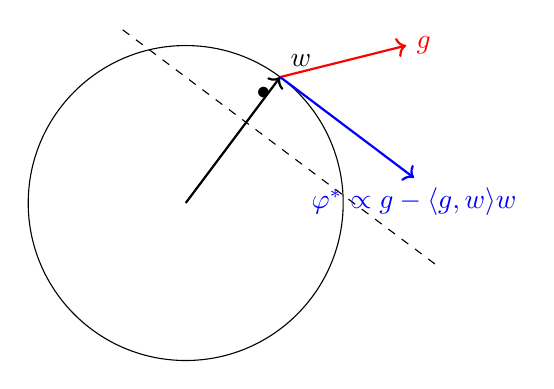
\begin{tikzpicture}[scale=2]
  \draw (0,0) circle (1);
  \draw[->,thick] (0,0)--(0.6,0.8) node[above right]{$w$};
  \draw[->,thick,red] (0.6,0.8)--(1.4,1.0) node[right]{$g$};
  \draw[dashed] (-0.4,1.1)--(1.6,-0.4);
  \draw[->,thick,blue] (0.6,0.8)--(1.45,0.16);
  \node[blue,below] at (1.45,0.16) {$\varphi^\ast \propto g-\inner{g}{w}w$};
  \node[below left] at (0.6,0.8){$\bullet$};
\end{tikzpicture}
\end{center}

\textbf{$\varphi^\ast$ 即把梯度 $g$ 投影到切空间。}

% ============================================================
\section{第七讲：正交方阵流形上的 Muon}\label{sec:orth}
% ============================================================

\subsection{问题表述}
$W\in\R^{n\times n}$，$W^\top W = WW^\top = I$。
\begin{equation}\label{eq:orth-prob}
\max_\Phi\;\tr(G^\top \Phi)\;\text{s.t.}\;\|\Phi\|_2=1,\;W^\top W = I,\;(W-\eta\Phi)^\top(W-\eta\Phi)=I.
\end{equation}

\subsection{一阶近似 = 切空间条件}
最后一个约束展开后，去掉 $O(\eta^2)$ 项，得
$W^\top \Phi + \Phi^\top W = 0$，即 $W^\top \Phi$ 是\textbf{反对称}矩阵——这就是 Stiefel/正交流形的切空间条件。

\subsection{待定系数法}
引入对称矩阵乘子 $\Lambda$：
$$\tr(G^\top\Phi) = \tr((G+W(\Lambda+\Lambda^\top))^\top \Phi) \le \|G+W(\Lambda+\Lambda^\top)\|_\nuc.$$
记 $X = \Lambda+\Lambda^\top$（任意对称矩阵），等号条件
$\Phi = \msign(G + WX)$。
剩下需要找到使 $W^\top\Phi$ 反对称的对称矩阵 $X$。

\subsection{方阵情形的闭式解}
利用 $\msign$ 的两个性质：
\begin{enumerate}[leftmargin=2em]
\item 对正交方阵 $W$：$W^\top \msign(M) = \msign(W^\top M)$；
\item $\msign$ 保持反对称性：$M$ 反对称 $\Rightarrow \msign(M)$ 反对称。
\end{enumerate}
故 $W^\top\Phi = \msign(W^\top G + X)$。要使其反对称，由于 $X$ 对称，需 $W^\top G + X$ 反对称，即
$X = -[W^\top G]_{\mathrm{sym}}$，其中 $[M]_{\mathrm{sym}}:=\tfrac{1}{2}(M+M^\top)$。

\begin{theorem}[正交方阵流形上的 Muon]\label{thm:orth-square}
当 $W$ 方阵正交时，最速下降方向为
\begin{equation}
\boxed{\quad\Phi^\ast = W\,\msign\!\left([W^\top G]_{\mathrm{skew}}\right)\quad,\qquad
[M]_{\mathrm{skew}}:=\tfrac{1}{2}(M-M^\top).}
\end{equation}
\end{theorem}

\begin{proof}
代入 $X = -[W^\top G]_{\mathrm{sym}}$：
$\Phi^\ast = \msign(G - W[W^\top G]_{\mathrm{sym}}) = W\,\msign(W^\top G - [W^\top G]_{\mathrm{sym}}) = W\,\msign([W^\top G]_{\mathrm{skew}}).$
\qed
\end{proof}

\subsection{具体算例}

\begin{example}[$2\times 2$ 旋转矩阵的 Muon 更新]\label{ex:orth-numeric}
取 $W = I$（视作零角度旋转）、$G = \begin{pmatrix}1 & 2\\ 3 & 4\end{pmatrix}$。

\textbf{第 1 步：算 $W^\top G = G$。}

\textbf{第 2 步：取反对称部分。}
$[G]_{\mathrm{skew}} = \tfrac{1}{2}(G - G^\top) = \tfrac{1}{2}\begin{pmatrix}0 & -1\\ 1 & 0\end{pmatrix} = \begin{pmatrix}0 & -1/2\\ 1/2 & 0\end{pmatrix}$.

\textbf{第 3 步：算 $\msign$。}
该矩阵记作 $M$，则 $M^\top M = \tfrac{1}{4}I$，$(M^\top M)^{1/2} = \tfrac{1}{2}I$，故
$\msign(M) = M\cdot 2 = \begin{pmatrix}0 & -1\\ 1 & 0\end{pmatrix}$.

\textbf{第 4 步：组装。}
$\Phi^\ast = I\cdot \begin{pmatrix}0 & -1\\ 1 & 0\end{pmatrix}$，正是\textbf{逆时针 90° 旋转}！

\textbf{解读}：在正交群 $O(2)$ 上，更新方向必须是"反对称的指数 $e^{tA}$ 在 $t=0$ 处的方向"，即"角速度方向"。所以 $\Phi^\ast$ 自然落到了旋转方向上。

\textbf{第 5 步：更新与回缩。}
$W - \eta\Phi^\ast = \begin{pmatrix}1 & -\eta\\ \eta & 1\end{pmatrix}$。这恰是 $\sqrt{1+\eta^2}\cdot R_\theta$（$\tan\theta = \eta$）。除以 $\sqrt{1+\eta^2}$ 即得真正的旋转矩阵——回缩干净利落。
\end{example}

\subsection{回缩到正交群}

记 $O = \msign([W^\top G]_{\mathrm{skew}})$（反对称矩阵）。则 $(W-\eta\Phi)^\top (W-\eta\Phi) = I + \eta^2 O^\top O$。当 $[W^\top G]_{\mathrm{skew}}$ 满秩时 $O^\top O = I$，只需除以 $\sqrt{1+\eta^2}$；不满秩时则更新规则要再做一次 $\msign$（投影到正交群）。利用 $(O^\top O)^2 = O^\top O$ 可化简：
\begin{equation}
W \leftarrow W(I-\eta O)\!\left(I - O^\top O + \frac{O^\top O}{\sqrt{1+\eta^2}}\right).
\end{equation}

% ============================================================
\section{第八讲：Stiefel 流形上的 Muon}\label{sec:stiefel}
% ============================================================

\subsection{困难何在}
设 $W\in\R^{n\times m}$，$n>m$。$W^\top W = I_m$ 但 $WW^\top \ne I_n$，故 $W^\top$ \textbf{无法吸收进 $\msign$}。$X$ 不再有简单闭式解。\cite{bernstein-orth} 把这一情形列为 open problem。给出两类数值算法。

\subsection{方法 A：不动点迭代}

由 $\msign(G+WX) = (G+WX)Q^{-1}$，$Q = ((G+WX)^\top(G+WX))^{1/2}$。把切空间方程 $W^\top\Phi + \Phi^\top W = 0$ 改写后，两侧乘 $Q$：
\begin{equation}\label{eq:stiefel-lyap}
\boxed{\quad QX + XQ = -2\,[Q W^\top G]_{\mathrm{sym}}\quad}
\end{equation}
这是关于 $X$ 的\textbf{连续型 Lyapunov 方程}，$Q$ 已知时是线性的。

\textbf{迭代格式}：
\begin{enumerate}[leftmargin=2em]
\item 初值 $X^{(0)} = -[W^\top G]_{\mathrm{sym}}$（方阵情形的解）。
\item 计算 $\Phi^{(k)} = \msign(G+WX^{(k)})$，得 $Q^{(k)} = (G+WX^{(k)})^\top \Phi^{(k)}$。
\item 解 \eqref{eq:stiefel-lyap} 得 $X^{(k+1)}$。
\item 收敛即停。
\end{enumerate}

\subsection{Lyapunov 方程的两种求解}

\textbf{思路 1（$\mcsgn$）}：
$X = \mcsgn\!\left(\!\begin{bmatrix}-Q & -[QW^\top G]_{\mathrm{sym}}\\ 0 & Q\end{bmatrix}\!\right)\!_{[:m,m:]}$
其中 $\mcsgn$ 是矩阵符号函数（特征值替换为 $\pm 1$）。可用 Newton--Schulz 高效计算。

\textbf{思路 2（SVD）}：
$Q$ 正定对称，$Q = V\Sigma V^\top$。\eqref{eq:stiefel-lyap} 变为
$\Sigma(V^\top XV) + (V^\top XV)\Sigma = -2 V^\top [QW^\top G]_{\mathrm{sym}} V$。
设 $S_{ij}=\sigma_i+\sigma_j$，则
$X = -2 V\!\left( (V^\top [QW^\top G]_{\mathrm{sym}} V) \oslash S \right)\!V^\top$，$\oslash$ 为 Hadamard 商。
\textbf{巧妙之处}：$Q$ 的特征分解等价于 $G+WX$ 的 SVD，所以一次 SVD 同时给出 $\msign(G+WX)$ 和 $X$。

\subsection{数值算例：$4\times 2$ Stiefel 流形}\label{sec:stiefel-numeric}

下面给出迭代法的实测运行结果。取
$$W = \begin{pmatrix}-0.627 & \;\;0.128 \\ \;\;0.204 & -0.594 \\ -0.334 & -0.789 \\ -0.674 & \;\;0.092\end{pmatrix},\quad
G = \begin{pmatrix}\;\;0.319 & -0.249 \\ \;\;1.462 & -2.060 \\ -0.322 & -0.384 \\ \;\;1.134 & -1.100\end{pmatrix}$$
（$W$ 满足 $W^\top W = I_2$，由对一个 $4\times 2$ 标准高斯矩阵做 QR 得到）。

执行第 \ref{sec:code} 讲给出的 \verb|muon_stiefel_svd| 函数，记每步的目标值 $\tr(G^\top \Phi^{(k)})$ 与切空间残差 $\|W^\top\Phi^{(k)}+(\Phi^{(k)})^\top W\|_F$：
$$
\begin{array}{c|cc}
k & \tr(G^\top \Phi^{(k)}) & \text{切空间残差} \\\hline
0  & 2.3592 & 1.12\times 10^{0} \\
1  & 2.4611 & 9.42\times 10^{-1} \\
3  & 2.5550 & 6.79\times 10^{-1} \\
5  & 2.7507 & 7.10\times 10^{-2} \\
8  & 2.7731 & 2.67\times 10^{-4} \\
10 & 2.7732 & 5.99\times 10^{-6} \\
12 & 2.7732 & 1.34\times 10^{-7} \\
\end{array}
$$
\textbf{观察}：(1) 目标值 $\tr(G^\top\Phi^{(k)})$ \emph{严格单调上升}（这正是约束最大化所期望的）；(2) 切空间残差几乎以\emph{超线性}速率降至机器精度。

\textbf{对比基准}：
\begin{itemize}[leftmargin=2em]
\item \emph{无约束最优}：$\tr(G^\top \msign(G)) = \|G\|_\nuc = 3.5541$（不满足切空间约束）。
\item \emph{初值（方阵闭式解照搬到非方阵）}：$2.3592$，比真正约束最优低约 $15\%$。
\item \emph{迭代收敛值}：$2.7732$。
\end{itemize}
非方阵 Stiefel 与方阵正交的差距正在于此——闭式解不再是真正的约束最优，必须迭代。

\subsection{方法 B：对偶梯度下降}\label{sec:dual}

\textbf{关键观察}：核范数的梯度是 $\msign$：$\nabla_M \|M\|_\nuc = \msign(M)$。
故对 $\|G+WX\|_\nuc$ 关于 $\Lambda$（$X = \Lambda+\Lambda^\top$）求梯度：
$$\nabla_\Lambda \|G+WX\|_\nuc = W^\top \msign(G+WX) + \msign(G+WX)^\top W = W^\top\Phi + \Phi^\top W.$$
\textbf{所以解切空间方程 $W^\top\Phi+\Phi^\top W=0$ 等价于求 $\|G+WX\|_\nuc$ 的（局部）极值！}

\subsubsection*{对偶上升的来源——拉格朗日对偶}
$$\max_{\|\Phi\|_2\le 1}\min_{\Lambda}\, \tr(G^\top\Phi) + \tr(\Lambda^\top(W^\top\Phi+\Phi^\top W))
= \min_\Lambda \|G+WX\|_\nuc.$$
（用 Minimax 定理交换 $\min,\max$。）即原问题的\textbf{对偶问题}就是核范数最小化。

\subsubsection*{对偶梯度下降 + 在线参数同步}
\begin{equation}\label{eq:dual-iter}
\boxed{
\begin{aligned}
\Phi &= \msign(G+WX),\\
W &\leftarrow W - \eta_1 \Phi,\\
X &\leftarrow X - \eta_2 (W^\top\Phi + \Phi^\top W).
\end{aligned}
}
\end{equation}
不需要内层完全收敛——$X$ 与 $W$ 同步更新即可。这正是 \emph{Modular Manifolds} \cite{tml-mm} 的用法。

\subsection{回缩}
若 $G+WX$ 满秩（数值上几乎总成立）：
$(W-\eta\Phi)^\top(W-\eta\Phi) = (1+\eta^2)I_m$，故只需归一化：
$W \leftarrow (W-\eta\Phi)/\sqrt{1+\eta^2}$。建议\emph{周期性}做 $W \leftarrow \msign(W)$ 把参数硬拉回 Stiefel 流形，且整个迭代建议 FP32 起步。

% ============================================================
\section{第九讲：谱球面上的 Muon}\label{sec:spec-sphere}
% ============================================================

\subsection{问题与一阶近似}

希望参数的谱范数恒为 $1$：
$\max_\Phi\,\tr(G^\top\Phi)$ s.t.\ $\|\Phi\|_2=1,\;\|W\|_2=1,\;\|W-\eta\Phi\|_2=1$。

由 SVD 的导数（见附录 A）：$\nabla_W\|W\|_2 = u_1 v_1^\top =: \Theta$（最大奇异向量外积）。一阶近似下两个谱范数条件等价于 $\tr(\Theta^\top\Phi) = 0$。

通用形式：
\begin{equation}
\max_\Phi\; \tr(G^\top\Phi)\quad\text{s.t.}\;\;\|\Phi\|_2=1,\; \tr(\Theta^\top\Phi)=0.
\end{equation}

\subsection{待定系数与不动点迭代}
$\tr(G^\top\Phi) \le \|G+\lambda\Theta\|_\nuc$，
$\Phi^\ast = \msign(G+\lambda\Theta)$。
$\lambda$ 是标量，但满足 $\tr(\Theta^\top\Phi)=0$ 仍是非线性方程。利用与 Stiefel 类似技巧：
\begin{equation}
\boxed{\quad\lambda = \frac{\tr(\Theta^\top \Phi Q) - \tr(\Theta^\top\Phi)\tr(Q)/m - \tr(\Theta^\top G)}{\tr(\Theta^\top \Theta)}\quad}
\end{equation}
其中 $Q = (G+\lambda\Theta)^\top \Phi$。代入初值 $\lambda^{(0)} = -\tr(\Theta^\top G)/\tr(\Theta^\top\Theta)$，反复迭代即可。

\subsection{对偶梯度下降视角}
由核范数梯度公式：
$\nabla_\lambda \|G+\lambda\Theta\|_\nuc = \tr(\Theta^\top \msign(G+\lambda\Theta)) = \tr(\Theta^\top\Phi)$。
所以解切空间方程 = 求 $\|G+\lambda\Theta\|_\nuc$ 关于 $\lambda$ 的最小值。可以做
$\Phi=\msign(G+\lambda\Theta)$，$W\leftarrow W-\eta_1\Phi$，$\lambda\leftarrow \lambda-\eta_2\tr(\Theta^\top\Phi)$。
形式上是 Muon 的一种\textbf{自适应权重衰减}。

\subsection{数值算例：$3\times 3$ 谱球面}\label{sec:spec-sphere-numeric}

取
$$W = \diag(1,\,0.7,\,0.3),\qquad G = \begin{pmatrix}1.007 & 0.360 & 0.510\\ 0.622 & 0.263 & 0.501\\ 0.500 & -0.026 & 0.805\end{pmatrix}.$$
$\|W\|_2 = 1$（顶奇异值唯一，$\sigma_2 = 0.7$ 与之分得很开），$\Theta = u_1 v_1^\top = e_1 e_1^\top = \begin{pmatrix}1 & 0 & 0\\ 0 & 0 & 0\\ 0 & 0 & 0\end{pmatrix}$。

\textbf{无约束基线}：$\|G\|_\nuc = 2.213$（即 $\msign(G)$ 与 $G$ 的内积上限）。但这违反切空间约束 $\tr(\Theta^\top \Phi) = 0$。

\textbf{对偶 GD（步长 $\eta_2 = 0.1$）}：解 $\min_\lambda \|G + \lambda\Theta\|_\nuc$，每步
$\lambda \leftarrow \lambda - 0.1 \cdot \tr(\Theta^\top\Phi)$。
$$
\begin{array}{c|cc|c}
\hline
k & \lambda & \|G+\lambda\Theta\|_\nuc & \tr(\Theta^\top\Phi)\;\text{（梯度）} \\\hline
0 & 0       & 2.213 & +0.991 \\
1 & -0.099  & 2.115 & +0.989 \\
2 & -0.198  & 2.017 & +0.987 \\
3 & -0.297  & 1.939 & +0.231 \\
4 & -0.320  & 1.934 & +0.205 \\
5 & -0.340  & 1.930 & +0.181 \\
8 & -0.388  & 1.922 & +0.126 \\
14 & -0.445 & 1.917 & +0.061 \\\hline
\multicolumn{2}{c|}{\text{解析最优}} & 1.915 & 0 \\\hline
\end{array}
$$

\textbf{解读}：
\begin{itemize}[leftmargin=2em]
\item \textbf{相变发生在 $k=3$}：$\lambda$ 越过某临界值后，第三个奇异值（$\sigma_3 \approx 0.097$）开始成为约束的活跃方向，$\msign$ 的 $\Theta$ 分量从 $\approx 0.99$ 跳到 $\approx 0.23$。这是核范数函数\textbf{分段线性}的具体表现——每段对应一组奇异值排序。
\item \textbf{第二段缓慢收敛}：进入 $k\ge 3$ 后，梯度幅值小（$\sim 0.1$），所以收敛慢。换句话说，分段函数不同段对应"快下降"和"慢下降"两个区域。
\item \textbf{14 步后收敛到 $1.917$}，与解析最优 $1.915$ 误差 $0.002$。再小步长可继续逼近。
\end{itemize}

\textbf{在最优点的奇异值}：$\sigma(G + \lambda^* \Theta) = (1.452,\,0.365,\,0.097)$。第三奇异值很小但严格非零，\textbf{说明最优解在光滑区内}（不是奇异值简并点）；故 $\Phi^* = \msign(G+\lambda^*\Theta)$ 良定义。

\begin{remark}[核范数函数的几何]
$\lambda \mapsto \|G + \lambda\Theta\|_\nuc$ 是 $\lambda$ 的\textbf{凸、分段线性}函数，分段处对应于 $G+\lambda\Theta$ 的某对奇异值相等或某个奇异值过零。最优 $\lambda^*$ 几乎必落在分段点上（即"棱"上）——这是所有 $\ell_1$ 类问题的典型行为。所以\textbf{对偶 GD 在最优点附近会震荡}（梯度跳变），需要逐步衰减步长 $\eta_k = \eta_0/\sqrt{k}$ 或采用 proximal 方法才能精确收敛。
\end{remark}

% ============================================================
\section{第十讲：对偶梯度下降的统一视角}\label{sec:dual-unified}
% ============================================================

回过头看，第 \ref{sec:stiefel} 与第 \ref{sec:spec-sphere} 讲都用到了同一个观察：
\begin{tcolorbox}[colback=green!3,colframe=green!50!black,title=\textbf{Modular Manifolds 核心观察}]
"\textbf{切空间方程}"恰好是某个\textbf{核范数目标的梯度等于零}的条件。所以解约束最速下降 $\Leftrightarrow$ 求核范数的极小值。
\end{tcolorbox}

通用模板：
\begin{tcolorbox}[colback=gray!5,colframe=gray!50!black]
\textbf{输入}：损失梯度 $G$，参数 $W$，约束 $\mathcal{C}$ 对应的切空间投影由乘子 $\lambda$ 参数化。\\
\textbf{算法}：
\begin{enumerate}[leftmargin=2em]
\item $\Phi \gets \msign(G + (\text{乘子 $\lambda$ 的线性项}))$
\item $W \gets W - \eta_1 \Phi$ \quad（再做一次 retraction 拉回 $\mathcal{C}$）
\item $\lambda \gets \lambda - \eta_2 \cdot (\text{切空间方程的左端})$
\end{enumerate}
\end{tcolorbox}

每步只比朴素 Muon 多一次几乎免费的乘子更新，没有内层迭代，工程实现简洁。

\subsection{为什么核范数自然出现？}
拉格朗日对偶：
$\max_{\rho(\Phi)\le 1}\min_\lambda\, \tr(G^\top\Phi)+\inner{\lambda}{(\text{切空间方程})}=\min_\lambda \rho^\ast(G+W\cdot\lambda)$，
其中 $\rho^\ast$ 是 $\rho$ 的对偶范数。谱范数的对偶就是核范数，故核范数出现是必然结果。

% ============================================================
\section{第十一讲：实现细节与参考代码}\label{sec:code}
% ============================================================

\subsection{精度问题}
\begin{itemize}[leftmargin=2em]
\item \textbf{Muon（无流形约束）}：可在 BF16 下做 Newton--Schulz，对 GPT-2/LLaMA 类模型实测稳定。
\item \textbf{流形约束情形}：建议 \textbf{FP32}，因为 $W^\top W = I$ 是 $m(m+1)/2$ 个等式约束，低精度下漂移很快。一般受约束的参数量小（少数 attention 头/projection），代价可接受。
\item \textbf{回缩}：除归一化外，建议每 $\sim 100$--$1000$ 步做一次 $W \leftarrow \msign(W)$ 把参数硬拉回流形。
\end{itemize}

\subsection{Stiefel 流形 Muon 参考实现}

\begin{lstlisting}
import numpy as np

def msign(g):
    u, s, vh = np.linalg.svd(g, full_matrices=False)
    return u @ np.diag(np.sign(s)) @ vh

def sym(x):  return (x + x.T) * 0.5
def skew(x): return (x - x.T) * 0.5

def muon_stiefel_svd(g, w, steps=10):
    """Stiefel 流形上的 Muon, 通过 SVD 路径求解 Lyapunov."""
    x = -sym(w.T @ g)              # 方阵情形的解作为初值
    for k in range(steps):
        z = g + w @ x
        u, s, vh = np.linalg.svd(z, full_matrices=False)
        phi = (u * np.sign(s)) @ vh
        # 一次 SVD 同时给出 msign 和 Lyapunov 方程的右端处理
        rhs = sym(z.T @ phi @ w.T @ g)
        x = -2 * vh.T @ ((vh @ rhs @ vh.T) /
                         (s + s[:, None] + 1e-12)) @ vh
    return phi

def muon_stiefel_dual(g, w, x, eta_inner=0.1):
    """Modular Manifolds 风格: 一次内层 dual ascent 步."""
    phi = msign(g + w @ x)
    grad_x = 2 * sym(w.T @ phi)    # = w^T phi + phi^T w
    x = x - eta_inner * grad_x
    return phi, x
\end{lstlisting}

\subsection{大模型训练中的实用建议}
\begin{enumerate}[leftmargin=2em]
\item \textbf{选择性应用}：只对真正需要正交/谱约束的层使用，例如分类头、codebook、SSM 转移矩阵。
\item \textbf{热身策略}：训练初期用普通 Muon，参数稳定后再切换到流形版。
\item \textbf{对偶版 vs 不动点版}：参数量大且只有少数受约束层 → 不动点版（精度高）；约束层很多或对计算敏感 → 对偶版（每步几乎免费）。
\item \textbf{动量}：与原版 Muon 一致，对 $G$ 做 Nesterov 动量平均后再做 $\msign$。
\end{enumerate}

% ============================================================
\section*{结语}
% ============================================================
\addcontentsline{toc}{section}{结语}

整个讲义沿着一条非常清晰的逻辑链：

\begin{center}
\begin{tikzpicture}[node distance=1cm, auto, every node/.style={align=center}]
\node[draw, rounded corners] (a) {最小作用量原理\\$\min L(w+\Delta w)$ s.t.\ $\rho(\Delta w)\le \eta$};
\node[draw, rounded corners, below=of a] (b) {一阶近似 + 范数选择\\$\Rightarrow$ SGD / SignSGD / Muon};
\node[draw, rounded corners, below=of b] (c) {增加流形约束\\切空间 + 待定系数};
\node[draw, rounded corners, below left=of c, xshift=1cm] (d) {解析闭式\\(球面、正交方阵)};
\node[draw, rounded corners, below=of c] (e) {不动点迭代\\(Stiefel、谱球面)};
\node[draw, rounded corners, below right=of c, xshift=-1cm] (f) {对偶梯度下降\\(Modular Manifolds)};
\draw[->] (a)--(b);
\draw[->] (b)--(c);
\draw[->] (c)--(d);
\draw[->] (c)--(e);
\draw[->] (c)--(f);
\end{tikzpicture}
\end{center}

无论是经典的球面 SGD、Muon，还是新近的 Stiefel/Modular Manifolds，背后都共享同一个数学骨架。\textbf{这种"骨架性"的认识比任何单一算法都更重要}——以后碰到新的流形约束（低秩、稀疏、群结构），都可以套用："写出切空间 $\to$ 列拉格朗日 $\to$ 找核范数对偶 $\to$ 不动点或对偶梯度下降"。

% ============================================================
\appendix
% ============================================================

\section{附录 A：常用矩阵恒等式备忘}

\begin{itemize}[leftmargin=2em]
\item \textbf{迹的循环不变性}：$\tr(AB)=\tr(BA)$，$\tr(A^\top B^\top)=\tr(B^\top A^\top)$。
\item \textbf{Frobenius 内积}：$\inner{A}{B}_\Frob = \tr(A^\top B) = \sum_{ij}A_{ij}B_{ij}$。
\item \textbf{对称-反对称分解}：$M = [M]_{\mathrm{sym}} + [M]_{\mathrm{skew}}$。
\item \textbf{$\msign$ 性质}：
  \begin{itemize}[leftmargin=1.5em]
  \item $\msign(M) = M(M^\top M)^{-1/2} = (MM^\top)^{-1/2} M$（列/行满秩时）。
  \item $\|M\|_\nuc = \tr(M^\top \msign(M)) = \tr((M^\top M)^{1/2})$。
  \item 方阵正交 $W$：$W^\top \msign(M) = \msign(W^\top M)$。
  \item $M$ 反对称 $\Rightarrow \msign(M)$ 反对称。
  \end{itemize}
\item \textbf{核范数梯度}：$\nabla_M \|M\|_\nuc = \msign(M)$（所有奇异值非零时）。
\item \textbf{谱范数梯度}：$\nabla_M \|M\|_2 = u_1 v_1^\top$（最大奇异值唯一时）。
\item \textbf{Hölder 不等式（矩阵版）}：$\tr(A^\top B) \le \|A\|_p \|B\|_q$，$1/p+1/q=1$；谱范数与核范数对偶（$p=\infty,q=1$）。
\end{itemize}

\section{附录 B：与相关研究方向的连接}

\subsection*{B.1 与各向同性 / Norm 层的联系}
线性层 $Y = XW$ 的特征视角下，$\Delta Y = -\eta X X^\top \nabla_Y L$。当 $XX^\top \approx I$（即输入各向同性），参数空间和特征空间的最速下降方向\textbf{一致}。BatchNorm/LayerNorm 等可视为对 $XX^\top \approx I$ 的强制施行——\textbf{都是希望优化器看到的几何更"标准"}。

\subsection*{B.2 与二阶优化器的联系}
Adam 的 $\hat v_t \approx \E[g^2]$ 可解释为 Hessian 的对角近似。Muon 的 $\msign$ 则相当于 polar factor，与 Shampoo、SOAP、DAWN 等更显式的二阶/谱方法属于同一谱系。流形约束下的 Muon（本讲义主题）可视为\textbf{二阶预条件 + 几何约束}双重视角下的统一。

\subsection*{B.3 BBP 相变与随机化方法}
当 $G$ 是噪声扰动下的"低秩 + 噪声"结构时，前 $k$ 个奇异值的稳定性由 BBP (Baik--Ben~Arous--Péché) 相变控制。这意味着 $\msign$ 在低 SNR 区域可能不稳定，需要加阻尼或仅对前 $k$ 大奇异值做处理——这正是头-尾谱分解类二阶优化器（如 DAWN）的设计动机。

\subsection*{B.4 测地线距离与本讲义优化主题的呼应}
第 \ref{sec:geom} 讲中介绍的 $k$-NN 图近似测地线距离的方法属于"流形学习"的经典工具。它和本讲义的优化主题共享同一种数学语言——\textbf{流形上的"局部欧氏，全局非欧"原则}：\textbf{数值上}，$k$-NN 图把局部欧氏距离拼成全局测地线距离；\textbf{优化上}，切空间投影把局部欧氏的最速下降方向拼成全局的流形下降轨迹。两者是同一思想在不同任务上的应用。

\section{附录 C：练习题}

\begin{exercise}\label{ex:msign-skew}
证明：若 $M\in\R^{n\times n}$ 反对称（$M^\top = -M$），则 $\msign(M)$ 也反对称。\\
\textbf{提示}：$M$ 反对称 $\Rightarrow M^\top M = -M^2$ 与 $M$ 可交换。
\end{exercise}

\begin{exercise}
对超球面上的 $L^p$ 范数最速下降，写出 $p\to\infty$ 的解，并解释其几何意义。
\end{exercise}

\begin{exercise}
对正交方阵流形（定理 \ref{thm:orth-square}），考虑 $G$ 是反对称矩阵的特殊情形，化简 $\Phi^\ast$ 的表达式。
\end{exercise}

\begin{exercise}
推导 Stiefel 流形上多重最大奇异值情形的迭代格式。
\end{exercise}

\begin{exercise}\label{ex:dual-conv}
对偶梯度下降 \eqref{eq:dual-iter} 的收敛性：证明在 $W$ 不变的假设下，$X$ 的更新会使 $\|G+WX\|_\nuc$ 单调下降（取充分小步长 $\eta_2$）。
\end{exercise}

\begin{exercise}\label{ex:geo-impl}
实现 $k$-NN 图测地线距离近似：
\begin{enumerate}[leftmargin=2em]
\item 在球面 $S^2$ 上随机采样 $N=500$ 个点；
\item 用 $k=10$ 构造邻近图；
\item 用 Dijkstra 求所有两两测地线距离的近似值，与精确值 $\arccos(\inner{p}{q})$ 比较；
\item 探究 $k$ 增大/减小时近似精度的变化。
\end{enumerate}
\end{exercise}

\begin{exercise}[实现题]
基于第 \ref{sec:code} 讲的代码，在 GPT-2 (124M) 上比较：(a) 普通 Muon；(b) Stiefel-Muon（仅 attention 输出 projection）；(c) Modular-Manifolds 版。报告训练曲线、wall-clock 与最终 perplexity。
\end{exercise}

% ============================================================
\begin{thebibliography}{99}
\bibitem{muon} K. Jordan et al., \emph{Muon: An optimizer for hidden layers in neural networks}, 2024.
\bibitem{bernstein-orth} J. Bernstein, \emph{Orthogonal Manifold}, blog post, 2024.
\bibitem{tml-mm} Thinking Machines Lab, \emph{Modular Manifolds}, 2025.
\bibitem{geo-summary} \emph{Unsupervised Opinion Summarization Using Approximate Geodesics}, 2022.
\bibitem{ref-1} \emph{流形上的最速下降：1.\ SGD + 超球面}, \url{https://spaces.ac.cn/archives/11196}.
\bibitem{ref-2} \emph{流形上的最速下降：2.\ Muon + 正交}, \url{https://spaces.ac.cn/archives/11215}.
\bibitem{ref-3} \emph{流形上的最速下降：3.\ Muon + Stiefel}, \url{https://spaces.ac.cn/archives/11221}.
\bibitem{ref-4} \emph{流形上的最速下降：4.\ Muon + 谱球面}, \url{https://spaces.ac.cn/archives/11241}.
\bibitem{ref-5} \emph{流形上的最速下降：5.\ 对偶梯度下降}, \url{https://spaces.ac.cn/archives/11388}.
\bibitem{ref-geo} \emph{从局部到全局：语义相似度的测地线距离}, \url{https://spaces.ac.cn/archives/9368}.
\end{thebibliography}

\end{document}
